\chapter{Résultats et discussion}\label{chap:EtudeExpe}
\mylocaltoc

\section{Introduction}\label{chap:EtudeExpe_Intro}
Lors des expériences réalisées lors de la caractérisation du réfrigérateur \textsc{Tacot}, il a été montré que le gradient axial de température dans le noyau thermoacoustique n'est pas linéaire, et que les températures ne sont pas homogènes le long de la direction transverse du noyau \echaf{figure ?}\cite{ramadan_design_2021}. Cet écart au comportement attendu, c'est-à-dire un gradient linéaire entre les côtés froid et ambiant du noyau thermoacoustique, ainsi qu'une température radiale uniforme sur la section du noyau thermoacoustique, implique la présence d'un écoulement moyen non nul et d'effets non-linéaires dans le réfrigérateur. Parmi les hypothèses formulées quant à la cause de ces disparités avec la théorie linéaire de Rott, plusieurs hypothèses peuvent être envisagées : vent acoustique, turbulence, formation de tourbillons, génération d'harmoniques supérieures, et convection naturelle. Parmi ces effets, peu d'études portent sur cette dernière, bien qu'il ait déjà été montré que le déclenchement de moteurs ou encore l'uniformité de température sur la section y étaient sensibles \cite{ross_influence_2003,  hireche_numerical_2019, ramadan_experimental_2018,  zhang_novel_2011}. Plusieurs paramètres sont étudiés pour quantifier la dépendance du comportement de la machine à la direction de la gravité. 

\section{\'Etude des performances}
Pour commencer cette étude expérimentale, une vue d'ensemble est adoptée. En faisant abstraction de la distribution de température non encore expliquée, des quantités telles que la capacité de refroidissement de l'échangeur froid $Q_f$ et la chaleur extraite par l'échangeur ambiant $Q_a$, le coefficient de performance $\COP=Q_f/W_e$ rapporté au coefficient de performance de Carnot $\COP_{\sf carnot} = T_f/(T_a-T_f)$ ou les température froide $T_f$ et ambiante $T_a$ sont relevées. Pour cette partie de l'étude, plusieurs hypothèses sont proposées : les températures sont supposées constantes sur la section du noyau, et les échangeurs sont considérés parfaits avec un flux thermique homogène sur la section. 

Dans cette étude, les quatre orientations définies sur les schémas de la figure~\ref{fig:OrientationCore} sont tour à tour mises en place. Pour chacune, des expériences sont réalisées en suivant le protocole défini dans la partie~\ref{chap:MesureAvecAcou}, cette fois en réglant les charges thermiques $\dot Q_f$ de \qtylist{50;100}{\watt}. Les résultats des expériences tracés sur les figures~\ref{fig:PerfConvNat_0W} à \ref{fig:PerfConvNat_100W} proviennent du tableau~\ref{tab:RecapResultExpe}.\medskip


%\begin{figure}[!ht]
%    \centering
%	\begin{subfigure}{.48\textwidth}
%		\centering
%		\external{fig_PerfConvNat_Tf}
%%        \externalremake
%        \begin{tikzpicture}[every mark/.append style={mark size=5pt}]
	\def\width{.9*\textwidth};
	\def\height{\width};
	
	\begin{axis}[width=\width,height=\height,
		grid=both,minor tick num=4, 
		grid style={line width=.1pt, draw=gray!10},
	    major grid style={line width=.2pt,draw=gray!50},
	    xmin=.1,xmax=3.8,
		xlabel={$DR$ [\unit{\percent}]},
		ylabel={$T_f$ [\unit{\kelvin}]},
		legend style = {at={(0,1.02)}, anchor=south west, rounded corners, legend columns=3,},
		legend cell align={left},
		legend entries={`\texttt{V1}', `\texttt{V2}', \textsc{DeltaEC}, `\texttt{H1}',  `\texttt{H2}', {\quad}, \qty{0}{\watt}, \qty{50}{\watt}, \qty{100}{\watt}}
	]
	
	\addlegendimage{only marks, mark=square*, color=MatlabBlue}
	\addlegendimage{only marks, mark=square, color=MatlabBlue}
	\addlegendimage{only marks, mark=oplus}
	\addlegendimage{only marks, mark=square*, color=MatlabOrange}
	\addlegendimage{only marks, mark=square, color=MatlabOrange}
	\addlegendimage{empty legend}
	\addlegendimage{only marks, mark=o}
	\addlegendimage{only marks, mark=diamond}
	\addlegendimage{only marks, mark=triangle}
	
	\addplot[only marks, mark=*,color=MatlabBlue] file {../fig/fig_PerfConvNat/data/V1_Tf_DR_Qc0.txt};%\addlegendentry{`\texttt{V1}'};
	\addplot[only marks, mark=o,color=MatlabBlue] file {../fig/fig_PerfConvNat/data/V2_Tf_DR_Qc0.txt};%\addlegendentry{`\texttt{V2}'};
	\addplot[only marks, mark=*,color=MatlabOrange] file {../fig/fig_PerfConvNat/data/H1_Tf_DR_Qc0.txt};%\addlegendentry{`\texttt{H1}'};
	\addplot[only marks, mark=o,color=MatlabOrange] file {../fig/fig_PerfConvNat/data/H2_Tf_DR_Qc0.txt};%\addlegendentry{`\texttt{H2}'};
	
	\addplot[only marks, mark=diamond*,color=MatlabBlue] file {../fig/fig_PerfConvNat/data/V1_Tf_DR_Qc50.txt};%\addlegendentry{`\texttt{V1}'};
	\addplot[only marks, mark=diamond,color=MatlabBlue] file {../fig/fig_PerfConvNat/data/V2_Tf_DR_Qc50.txt};%\addlegendentry{`\texttt{V2}'};
	\addplot[only marks, mark=diamond*,color=MatlabOrange] file {../fig/fig_PerfConvNat/data/H1_Tf_DR_Qc50.txt};%\addlegendentry{`\texttt{H1}'};
	\addplot[only marks, mark=diamond,color=MatlabOrange] file {../fig/fig_PerfConvNat/data/H2_Tf_DR_Qc50.txt};%\addlegendentry{`\texttt{H2}'};
	
	\addplot[only marks, mark=triangle*,color=MatlabBlue] file {../fig/fig_PerfConvNat/data/V1_Tf_DR_Qc100.txt};%\addlegendentry{`\texttt{V1}'};
	\addplot[only marks, mark=triangle,color=MatlabBlue] file {../fig/fig_PerfConvNat/data/V2_Tf_DR_Qc100.txt};%\addlegendentry{`\texttt{V2}'};
	\addplot[only marks, mark=triangle*,color=MatlabOrange] file {../fig/fig_PerfConvNat/data/H1_Tf_DR_Qc100.txt};%\addlegendentry{`\texttt{H1}'};
	\addplot[only marks, mark=triangle,color=MatlabOrange] file {../fig/fig_PerfConvNat/data/H2_Tf_DR_Qc100.txt};%\addlegendentry{`\texttt{H2}'};
	\end{axis}
\end{tikzpicture}
%		\caption{}
%		\label{fig:PerfConvNat_Tf}
%	\end{subfigure}%
%	\begin{subfigure}{.48\textwidth}
%		\centering
%		\external{fig_PerfConvNat_Ta}
%%        \externalremake
%        \begin{tikzpicture}[every mark/.append style={mark size=5pt}]
	\def\width{.9*\textwidth};
	\def\height{\width};
	
	\begin{axis}[width=\width,height=\height,
		grid=both,minor tick num=4, 
		grid style={line width=.1pt, draw=gray!10},
	    major grid style={line width=.2pt,draw=gray!50},
	    xmin=.1,xmax=3.8,
		xlabel={$DR$ [\unit{\percent}]},
		ylabel={$T_a$ [\unit{\kelvin}]},
		legend style = {at={(.5,1.05)}, anchor=south, rounded corners, legend columns=2}
	]
	
	\addplot[only marks, mark=*, color=MatlabBlue] file {../fig/fig_PerfConvNat/data/V1_Ta_DR_Qc0.txt};%\addlegendentry{`\texttt{V1}'};
	\addplot[only marks, mark=o, color=MatlabBlue] file {../fig/fig_PerfConvNat/data/V2_Ta_DR_Qc0.txt};%\addlegendentry{`\texttt{V2}'};
	\addplot[only marks, mark=*,color=MatlabOrange] file {../fig/fig_PerfConvNat/data/H1_Ta_DR_Qc0.txt};%\addlegendentry{`\texttt{H1}'};
	\addplot[only marks, mark=o,color=MatlabOrange] file {../fig/fig_PerfConvNat/data/H2_Ta_DR_Qc0.txt};%\addlegendentry{`\texttt{H2}'};
	
	\addplot[only marks, mark=diamond*,color=MatlabBlue] file {../fig/fig_PerfConvNat/data/V1_Ta_DR_Qc50.txt};%\addlegendentry{`\texttt{V1}'};
	\addplot[only marks, mark=diamond,color=MatlabBlue] file {../fig/fig_PerfConvNat/data/V2_Ta_DR_Qc50.txt};%\addlegendentry{`\texttt{V2}'};
	\addplot[only marks, mark=diamond*,color=MatlabOrange] file {../fig/fig_PerfConvNat/data/H1_Ta_DR_Qc50.txt};%\addlegendentry{`\texttt{H1}'};
	\addplot[only marks, mark=diamond,color=MatlabOrange] file {../fig/fig_PerfConvNat/data/H2_Ta_DR_Qc50.txt};%\addlegendentry{`\texttt{H2}'};
	
	\addplot[only marks, mark=triangle*,color=MatlabBlue] file {../fig/fig_PerfConvNat/data/V1_Ta_DR_Qc100.txt};%\addlegendentry{`\texttt{V1}'};
	\addplot[only marks, mark=triangle,color=MatlabBlue] file {../fig/fig_PerfConvNat/data/V2_Ta_DR_Qc100.txt};%\addlegendentry{`\texttt{V2}'};
	\addplot[only marks, mark=triangle*,color=MatlabOrange] file {../fig/fig_PerfConvNat/data/H1_Ta_DR_Qc100.txt};%\addlegendentry{`\texttt{H1}'};
	\addplot[only marks, mark=triangle,color=MatlabOrange] file {../fig/fig_PerfConvNat/data/H2_Ta_DR_Qc100.txt};%\addlegendentry{`\texttt{H2}'};
	\end{axis}
\end{tikzpicture}
%		\caption{}
%		\label{fig:PerfConvNat_Ta}
%	\end{subfigure}
%	
%	\vspace{.75cm}
%	
%	\begin{subfigure}{.48\textwidth}
%		\centering
%		\external{fig_PerfConvNat_Qa}
%%        \externalremake
%        \input{../fig/fig_PerfConvNat/tex/fig_PerfConvNat_Qa}
%		\caption{}
%		\label{fig:PerfConvNat_Qa}
%	\end{subfigure}%
%	\begin{subfigure}{.48\textwidth}
%		\centering
%		\external{fig_PerfConvNat_COP}
%%        \externalremake
%        \begin{tikzpicture}[every mark/.append style={mark size=5pt, line width=2pt}]
	\def\width{.9*\textwidth};
	\def\height{\width};
	
	\begin{axis}[width=\width,height=\height,
		grid=both,minor tick num=4, 
		grid style={line width=.1pt, draw=gray!10},
	    major grid style={line width=.2pt,draw=gray!50},
	    xmin=.1,xmax=3.8,
		xlabel={$DR$ [\unit{\percent}]},
		ylabel={$\COP$ [\unit{\percent}]},
		legend style = {at={(.01,.99)}, anchor=north west, rounded corners, legend columns=2},
%		legend entries={`\texttt{V1}', `\texttt{V2}', `\texttt{H1}', `\texttt{H2}', \qty{0}{\watt}, \qty{50}{\watt}, \qty{100}{\watt}, \textsc{DeltaEC}}
	]
	
%	\addlegendimage{only marks, mark=square*,color=MatlabBlue}
%	\addlegendimage{only marks, mark=square,color=MatlabBlue}
%	\addlegendimage{only marks, mark=square*,color=MatlabOrange}
%	\addlegendimage{only marks, mark=square,color=MatlabOrange}
%	\addlegendimage{only marks, mark=o}
%	\addlegendimage{only marks, mark=diamond}
%	\addlegendimage{only marks, mark=triangle}
%	\addlegendimage{only marks, mark=oplus}
	
	\addplot[only marks, mark=triangle*,color=MatlabBlue] file {../fig/fig_PerfConvNat/data/V1_COP_DR_Qc0.txt};%\addlegendentry{`\texttt{V1}'};
	\addplot[only marks, mark=triangle,color=MatlabBlue] file {../fig/fig_PerfConvNat/data/V2_COP_DR_Qc0.txt};%\addlegendentry{`\texttt{V2}'};
	\addplot[only marks, mark=triangle*,color=MatlabOrange] file {../fig/fig_PerfConvNat/data/H1_COP_DR_Qc0.txt};%\addlegendentry{`\texttt{H1}'};
	\addplot[only marks, mark=triangle,color=MatlabOrange] file {../fig/fig_PerfConvNat/data/H2_COP_DR_Qc0.txt};%\addlegendentry{`\texttt{H2}'};
	
	\addplot[only marks, mark=diamond*,color=MatlabBlue] file {../fig/fig_PerfConvNat/data/V1_COP_DR_Qc50.txt};%\addlegendentry{`\texttt{V1}'};
	\addplot[only marks, mark=diamond,color=MatlabBlue] file {../fig/fig_PerfConvNat/data/V2_COP_DR_Qc50.txt};%\addlegendentry{`\texttt{V2}'};
	\addplot[only marks, mark=diamond*,color=MatlabOrange] file {../fig/fig_PerfConvNat/data/H1_COP_DR_Qc50.txt};%\addlegendentry{`\texttt{H1}'};
	\addplot[only marks, mark=diamond,color=MatlabOrange] file {../fig/fig_PerfConvNat/data/H2_COP_DR_Qc50.txt};%\addlegendentry{`\texttt{H2}'};
	
	\addplot[only marks, mark=pentagon*,color=MatlabBlue] file {../fig/fig_PerfConvNat/data/V1_COP_DR_Qc100.txt};%\addlegendentry{`\texttt{V1}'};
	\addplot[only marks, mark=pentagon,color=MatlabBlue] file {../fig/fig_PerfConvNat/data/V2_COP_DR_Qc100.txt};%\addlegendentry{`\texttt{V2}'};
	\addplot[only marks, mark=pentagon*,color=MatlabOrange] file {../fig/fig_PerfConvNat/data/H1_COP_DR_Qc100.txt};%\addlegendentry{`\texttt{H1}'};
	\addplot[only marks, mark=pentagon,color=MatlabOrange] file {../fig/fig_PerfConvNat/data/H2_COP_DR_Qc100.txt};%\addlegendentry{`\texttt{H2}'};
	\end{axis}
\end{tikzpicture}
%		\caption{}
%		\label{fig:PerfConvNat_COP}
%	\end{subfigure}	     
%    \caption{Influence de la convection naturelle sur les performances sur différents indicateur : \subref{fig:PerfConvNat_Tf} température froide $T_f$, \subref{fig:PerfConvNat_Ta} température ambiante~$T_a$, \subref{fig:PerfConvNat_Qa} quantité de chaleur extraite du côté ambiant $\dot Q_a$, et \subref{fig:PerfConvNat_COP} le coefficient de performance rapporté à Carnot. Les températures indiquées représentent l'évolution depuis l'état avant le démarrage des sources acoustiques. Les couleurs indiquent l'orientation ; le remplissage, si le résultat est obtenu expérimentalement ou par une simulation \textsc{DeltaEC} ; la forme du marqueur, la puissance thermique fournie à l'échangeur froid $Q_f$.\echaf{ajouter valeurs DeltaEC}}
%    \label{fig:PerfConvNat}
%\end{figure}

\begin{figure}[!ht]
    \centering
	\begin{subfigure}{.48\textwidth}
		\centering
		\external{fig_PerfConvNat_Tf_0W}
%        \externalremake
        \begin{tikzpicture}[every mark/.append style={line width=2pt}]
	\def\width{.9*\textwidth};
	\def\height{\width};
	
	\begin{axis}[width=\width,height=\height,
		grid=both,minor tick num=4, 
		grid style={line width=.1pt, draw=gray!10},
	    major grid style={line width=.2pt,draw=gray!50},
	    xmin=.1,xmax=3.8,
		xlabel={$DR$ [\unit{\percent}]},
		ylabel={$T_f$ [\unit{\kelvin}]},
		legend style = {at={(.98,.98)}, anchor=north east, rounded corners, legend columns=2,},
		legend cell align={left},
%		legend entries={`\texttt{V1}', `\texttt{V2}',
%		`\texttt{H1}', `\texttt{H2}',
%		{Expé.}, {Simu.}
%		}
	]
	
	\addplot[only marks, mark=*,color=Plasma1, mark size=5pt] file {../fig/fig_PerfConvNat/data/V1_Tf_DR_Qc0.txt};\addlegendentry{`\texttt{V1}'};
	\addplot[only marks, mark=*,color=Plasma25, mark size=4pt] file {../fig/fig_PerfConvNat/data/V2_Tf_DR_Qc0.txt};\addlegendentry{`\texttt{V2}'};
	\addplot[only marks, mark=*,color=Plasma50, mark size=3pt] file {../fig/fig_PerfConvNat/data/H1_Tf_DR_Qc0.txt};\addlegendentry{`\texttt{H1}'};
	\addplot[only marks, mark=*,color=Plasma75, mark size=2pt] file {../fig/fig_PerfConvNat/data/H2_Tf_DR_Qc0.txt};\addlegendentry{`\texttt{H2}'};
	
	\addlegendimage{only marks, mark=square*, mark size=5pt}
	\addlegendentry{Expé.}
	
	\addlegendimage{only marks, mark=square, mark size=5pt}
	\addlegendentry{Simu.}

	\end{axis}
\end{tikzpicture}
		\caption{}
		\label{fig:PerfConvNat_0W_Tf}
	\end{subfigure}%
	\begin{subfigure}{.48\textwidth}
		\centering
		\external{fig_PerfConvNat_0W_Ta}
%        \externalremake
        \input{../fig/fig_PerfConvNat/tex/fig_PerfConvNat_0W_Ta}
		\caption{}
		\label{fig:PerfConvNat_0W_Ta}
	\end{subfigure}
	
	\vspace{.75cm}
	
	\begin{subfigure}{.48\textwidth}
		\centering
		\external{fig_PerfConvNat_0W_Qa}
%        \externalremake
        \begin{tikzpicture}[every mark/.append style={mark size=5pt, line width=2pt}]
	\def\width{.9*\textwidth};
	\def\height{\width};
	
	\begin{axis}[width=\width,height=\height,
		grid=both,minor tick num=4, 
		grid style={line width=.1pt, draw=gray!10},
	    major grid style={line width=.2pt,draw=gray!50},
	    xmin=.1,xmax=3.8,
		xlabel={$DR$ [\unit{\percent}]},
		ylabel={$\dot Q_a$ [\unit{\watt}]},
		legend style = {at={(.05,.95)}, anchor=north west, rounded corners, legend columns=2}
	]
	\addplot[only marks, mark=*,color=MatlabBlue] file {../fig/fig_PerfConvNat/data/V1_Qa_DR_Qc0.txt};%\addlegendentry{`\texttt{V1}'};
	\addplot[only marks, mark=*,color=MatlabOrange] file {../fig/fig_PerfConvNat/data/V2_Qa_DR_Qc0.txt};%\addlegendentry{`\texttt{V2}'};
	\addplot[only marks, mark=*,color=MatlabYellow] file {../fig/fig_PerfConvNat/data/H1_Qa_DR_Qc0.txt};%\addlegendentry{`\texttt{H1}'};
	\addplot[only marks, mark=*,color=MatlabPurple] file {../fig/fig_PerfConvNat/data/H2_Qa_DR_Qc0.txt};%\addlegendentry{`\texttt{H2}'};
	
	
	\end{axis}
\end{tikzpicture}
		\caption{}
		\label{fig:PerfConvNat_0W_Qa}
	\end{subfigure}%
%	\begin{subfigure}{.48\textwidth}
%		\centering
%		\external{fig_PerfConvNat_0W_COP}
%%        \externalremake
%        \input{../fig/fig_PerfConvNat/tex/fig_PerfConvNat_0W_COP}
%		\caption{}
%		\label{fig:PerfConvNat_0W_COP}
%	\end{subfigure}	     
    \caption{Influence de la convection naturelle sur les performances sur différents indicateur, pour une charge thermique $Q_f=\qty{0}{\watt}$ : \subref{fig:PerfConvNat_0W_Tf} température froide $T_f$, \subref{fig:PerfConvNat_0W_Ta} température ambiante~$T_a$, et \subref{fig:PerfConvNat_0W_Qa} quantité de chaleur extraite du côté ambiant $\dot Q_a$. Les températures indiquées représentent l'évolution depuis l'état avant le démarrage des sources acoustiques. Les couleurs indiquent l'orientation et le remplissage, si le résultat est obtenu expérimentalement ou par une simulation \textsc{DeltaEC}.\echaf{ajouter valeurs DeltaEC}}
    \label{fig:PerfConvNat_0W}
\end{figure}

\begin{figure}[!ht]
    \centering
	\begin{subfigure}{.48\textwidth}
		\centering
		\external{fig_PerfConvNat_50W_Tf}
%        \externalremake
        \begin{tikzpicture}[every mark/.append style={line width=2pt}]
	\def\width{.9*\textwidth};
	\def\height{\width};
	
	\begin{axis}[width=\width,height=\height,
		grid=both,minor tick num=4, 
		grid style={line width=.1pt, draw=gray!10},
	    major grid style={line width=.2pt,draw=gray!50},
	    xmin=.1,xmax=3.8,
		xlabel={$DR$ [\unit{\percent}]},
		ylabel={$T_f$ [\unit{\kelvin}]},
		legend style = {at={(.02,.02)}, anchor=south west, rounded corners, legend columns=2,},
		legend cell align={left},
%		legend entries={`\texttt{V1}', `\texttt{V2}',
%		`\texttt{H1}', `\texttt{H2}',
%		{Expé.}, {Simu.}
%		}
	]

		
	\addplot[only marks, mark=triangle*,color=Plasma1, mark size=5pt] file {../fig/fig_PerfConvNat/data/V1_Tf_DR_Qc50.txt};\addlegendentry{`\texttt{V1}'};
	\addplot[only marks, mark=triangle*,color=Plasma29, mark size=4pt] file {../fig/fig_PerfConvNat/data/V2_Tf_DR_Qc50.txt};\addlegendentry{`\texttt{V2}'};
	\addplot[only marks, mark=triangle*,color=Plasma57, mark size=3pt] file {../fig/fig_PerfConvNat/data/H1_Tf_DR_Qc50.txt};\addlegendentry{`\texttt{H1}'};
	\addplot[only marks, mark=triangle*,color=Plasma85, mark size=2pt] file {../fig/fig_PerfConvNat/data/H2_Tf_DR_Qc50.txt};\addlegendentry{`\texttt{H2}'};
	
		
	\addlegendimage{only marks, mark=square*, mark size=5pt}
	\addlegendentry{Expé.}
	
	\addlegendimage{only marks, mark=square, mark size=5pt}
	\addlegendentry{Simu.}
	
	
	\end{axis}
\end{tikzpicture}
		\caption{}
		\label{fig:PerfConvNat_50W_Tf}
	\end{subfigure}%
	\begin{subfigure}{.48\textwidth}
		\centering
		\external{fig_PerfConvNat_50W_Ta}
%        \externalremake
        \begin{tikzpicture}[every mark/.append style={line width=2pt}]
	\def\width{.9*\textwidth};
	\def\height{\width};
	
	\begin{axis}[width=\width,height=\height,
		grid=both,minor tick num=4, 
		grid style={line width=.1pt, draw=gray!10},
	    major grid style={line width=.2pt,draw=gray!50},
	    xmin=.1,xmax=3.8,
		xlabel={$DR$ [\unit{\percent}]},
		ylabel={$T_a$ [\unit{\kelvin}]},
		legend style = {at={(.5,1.05)}, anchor=south, rounded corners, legend columns=2}
	]
	
	
	\addplot[only marks, mark=triangle*,color=Plasma1, mark size=5pt] file {../fig/fig_PerfConvNat/data/V1_Ta_DR_Qc50.txt};%\addlegendentry{`\texttt{V1}'};
	\addplot[only marks, mark=triangle*,color=Plasma29, mark size=4pt] file {../fig/fig_PerfConvNat/data/V2_Ta_DR_Qc50.txt};%\addlegendentry{`\texttt{V2}'};
	\addplot[only marks, mark=triangle*,color=Plasma57, mark size=3pt] file {../fig/fig_PerfConvNat/data/H1_Ta_DR_Qc50.txt};%\addlegendentry{`\texttt{H1}'};
	\addplot[only marks, mark=triangle*,color=Plasma85, mark size=2pt] file {../fig/fig_PerfConvNat/data/H2_Ta_DR_Qc50.txt};%\addlegendentry{`\texttt{H2}'};
	
	\end{axis}
\end{tikzpicture}
		\caption{}
		\label{fig:PerfConvNat_50W_Ta}
	\end{subfigure}
	
	\vspace{.75cm}
	
	\begin{subfigure}{.48\textwidth}
		\centering
		\external{fig_PerfConvNat_50W_Qa}
%        \externalremake
        \begin{tikzpicture}[every mark/.append style={line width=2pt}]
	\def\width{.9*\textwidth};
	\def\height{\width};
	
	\begin{axis}[width=\width,height=\height,
		grid=both,minor tick num=4, 
		grid style={line width=.1pt, draw=gray!10},
	    major grid style={line width=.2pt,draw=gray!50},
	    xmin=.1,xmax=3.8,
		xlabel={$DR$ [\unit{\percent}]},
		ylabel={$\dot Q_a$ [\unit{\watt}]},
		legend style = {at={(.05,.95)}, anchor=north west, rounded corners, legend columns=2}
	]
	
		
	\addplot[only marks, mark=triangle*,color=Plasma1, mark size=5pt] file {../fig/fig_PerfConvNat/data/V1_Qa_DR_Qc50.txt};%\addlegendentry{`\texttt{V1}'};
	\addplot[only marks, mark=triangle*,color=Plasma29, mark size=4pt] file {../fig/fig_PerfConvNat/data/V2_Qa_DR_Qc50.txt};%\addlegendentry{`\texttt{V2}'};
	\addplot[only marks, mark=triangle*,color=Plasma57, mark size=3pt] file {../fig/fig_PerfConvNat/data/H1_Qa_DR_Qc50.txt};%\addlegendentry{`\texttt{H1}'};
	\addplot[only marks, mark=triangle*,color=Plasma85, mark size=2pt] file {../fig/fig_PerfConvNat/data/H2_Qa_DR_Qc50.txt};%\addlegendentry{`\texttt{H2}'};
	
	\end{axis}
\end{tikzpicture}
		\caption{}
		\label{fig:PerfConvNat_50W_Qa}
	\end{subfigure}%
	\begin{subfigure}{.48\textwidth}
		\centering
		\external{fig_PerfConvNat_50W_COP}
%        \externalremake
        \begin{tikzpicture}[every mark/.append style={line width=2pt}]
	\def\width{.9*\textwidth};
	\def\height{\width};
	
	\begin{axis}[width=\width,height=\height,
		grid=both,minor tick num=4, 
		grid style={line width=.1pt, draw=gray!10},
	    major grid style={line width=.2pt,draw=gray!50},
	    xmin=.1, xmax=3.8,
	    ymin=2.5, ymax=6.5,
		xlabel={$DR$ [\unit{\percent}]},
		ylabel={$\COP$ [\unit{\percent}]},
		legend style = {at={(.01,.99)}, anchor=north west, rounded corners, legend columns=2},
%		legend entries={`\texttt{V1}', `\texttt{V2}', `\texttt{H1}', `\texttt{H2}', \qty{0}{\watt}, \qty{50}{\watt}, \qty{100}{\watt}, \textsc{DeltaEC}}
	]

	
	\addplot[only marks, mark=triangle*,color=Plasma1, mark size=5pt] file {../fig/fig_PerfConvNat/data/V1_COP_DR_Qc50.txt};%\addlegendentry{`\texttt{V1}'};
	\addplot[only marks, mark=triangle*,color=Plasma28, mark size=4pt] file {../fig/fig_PerfConvNat/data/V2_COP_DR_Qc50.txt};%\addlegendentry{`\texttt{V2}'};
	\addplot[only marks, mark=triangle*,color=Plasma57, mark size=3pt] file {../fig/fig_PerfConvNat/data/H1_COP_DR_Qc50.txt};%\addlegendentry{`\texttt{H1}'};
	\addplot[only marks, mark=triangle*,color=Plasma85, mark size=2pt] file {../fig/fig_PerfConvNat/data/H2_COP_DR_Qc50.txt};%\addlegendentry{`\texttt{H2}'};
	
	\end{axis}
\end{tikzpicture}
		\caption{}
		\label{fig:PerfConvNat_50W_COP}
	\end{subfigure}	     
    \caption{Influence de la convection naturelle sur les performances sur différents indicateur, pour une charge thermique $Q_f=\qty{50}{\watt}$ : \subref{fig:PerfConvNat_50W_Tf} température froide $T_f$, \subref{fig:PerfConvNat_50W_Ta} température ambiante~$T_a$, \subref{fig:PerfConvNat_50W_Qa} quantité de chaleur extraite du côté ambiant $\dot Q_a$, et \subref{fig:PerfConvNat_50W_COP} coefficient de performance rapporté à Carnot. Les températures indiquées représentent l'évolution depuis l'état avant le démarrage des sources acoustiques. Les couleurs indiquent l'orientation et le remplissage, si le résultat est obtenu expérimentalement ou par une simulation \textsc{DeltaEC}.\echaf{ajouter valeurs DeltaEC}}
    \label{fig:PerfConvNat_50W}
\end{figure}

\begin{figure}[!ht]
    \centering
	\begin{subfigure}{.48\textwidth}
		\centering
		\external{fig_PerfConvNat_100W_Tf}
%        \externalremake
        \begin{tikzpicture}[every mark/.append style={mark size=5pt, line width=2pt}]
	\def\width{.9*\textwidth};
	\def\height{\width};
	
	\begin{axis}[width=\width,height=\height,
		grid=both,minor tick num=4, 
		grid style={line width=.1pt, draw=gray!10},
	    major grid style={line width=.2pt,draw=gray!50},
	    xmin=.1,xmax=3.8,
		xlabel={$DR$ [\unit{\percent}]},
		ylabel={$T_f$ [\unit{\kelvin}]},
		legend style = {at={(0,1.02)}, anchor=south west, rounded corners, legend columns=4,},
		legend cell align={left},
		legend entries={`\texttt{V1}', `\texttt{V2}',
		`\texttt{H1}', `\texttt{H2}',
		{Expé.}, {Simu.}
		}
	]
	
	\addlegendimage{only marks, mark=diamond*, color=MatlabBlue}
	\addlegendimage{only marks, mark=diamond*, color=MatlabOrange}
	
	\addlegendimage{only marks, mark=diamond*, color=MatlabYellow}
	\addlegendimage{only marks, mark=diamond*, color=MatlabPurple}
	
	\addlegendimage{only marks, mark=square*}
	\addlegendimage{only marks, mark=square}

		
	\addplot[only marks, mark=diamond*,color=MatlabBlue] file {../fig/fig_PerfConvNat/data/V1_Tf_DR_Qc100.txt};%\addlegendentry{`\texttt{V1}'};
	\addplot[only marks, mark=diamond*,color=MatlabOrange] file {../fig/fig_PerfConvNat/data/V2_Tf_DR_Qc100.txt};%\addlegendentry{`\texttt{V2}'};
	\addplot[only marks, mark=diamond*,color=MatlabYellow] file {../fig/fig_PerfConvNat/data/H1_Tf_DR_Qc100.txt};%\addlegendentry{`\texttt{H1}'};
	\addplot[only marks, mark=diamond*,color=MatlabPurple] file {../fig/fig_PerfConvNat/data/H2_Tf_DR_Qc100.txt};%\addlegendentry{`\texttt{H2}'};
	\end{axis}
\end{tikzpicture}
		\caption{}
		\label{fig:PerfConvNat_100W_Tf}
	\end{subfigure}%
	\begin{subfigure}{.48\textwidth}
		\centering
		\external{fig_PerfConvNat_100W_Ta}
%        \externalremake
        \input{../fig/fig_PerfConvNat/tex/fig_PerfConvNat_100W_Ta}
		\caption{}
		\label{fig:PerfConvNat_100W_Ta}
	\end{subfigure}
	
	\vspace{.75cm}
	
	\begin{subfigure}{.48\textwidth}
		\centering
		\external{fig_PerfConvNat_100W_Qa}
%        \externalremake
        \input{../fig/fig_PerfConvNat/tex/fig_PerfConvNat_100W_Qa}
		\caption{}
		\label{fig:PerfConvNat_100W_Qa}
	\end{subfigure}%
	\begin{subfigure}{.48\textwidth}
		\centering
		\external{fig_PerfConvNat_50W_COP}
%        \externalremake
        \input{../fig/fig_PerfConvNat/tex/fig_PerfConvNat_100W_COP}
		\caption{}
		\label{fig:PerfConvNat_100W_COP}
	\end{subfigure}	     
    \caption{Influence de la convection naturelle sur les performances sur différents indicateur, pour une charge thermique $Q_f=\qty{100}{\watt}$ : \subref{fig:PerfConvNat_100W_Tf} température froide $T_f$, \subref{fig:PerfConvNat_100W_Ta} température ambiante~$T_a$, \subref{fig:PerfConvNat_100W_Qa} quantité de chaleur extraite du côté ambiant $\dot Q_a$, et \subref{fig:PerfConvNat_100W_COP} le coefficient de performance rapporté à Carnot. Les températures indiquées représentent l'évolution depuis l'état avant le démarrage des sources acoustiques. Les couleurs indiquent l'orientation et le remplissage, si le résultat est obtenu expérimentalement ou par une simulation \textsc{DeltaEC}.\echaf{ajouter valeurs DeltaEC}}
    \label{fig:PerfConvNat_100W}
\end{figure}

La première observation concerne les températures atteintes aux deux extrémités du noyau, représentées sur les figures \ref{fig:PerfConvNat_0W_Tf}-\subref{fig:PerfConvNat_0W_Ta}, \ref{fig:PerfConvNat_50W_Tf}-\subref{fig:PerfConvNat_50W_Ta} et \ref{fig:PerfConvNat_100W_Tf}-\subref{fig:PerfConvNat_100W_Ta}. La température froide $T_f$, de manière générale, est plus basse quand le \textit{drive ratio} augmente. La température du côté ambiant est, quant à elle, relativement constante quel que soit le \textit{drive ratio} avec un écart de l'ordre de \qty{10}{\degreeCelsius}. Cette constance est expliqué par les échanges thermiques avec l'échangeur voisin.\smallskip

L'échangeur ambiant extrait la chaleur des volumes élémentaires de gaz qui oscillent à son voisinage. Il est donc attendu de voir la chaleur extraite par cet échangeur augmenter avec le \textit{drive ratio}. Comme attendu la tendance montrée sur les figures~\ref{fig:PerfConvNat_0W_Qa} le montre. \echaf{finir}


%\begin{figure}[!ht]
%    \centering
%	\begin{subfigure}[b]{.48\textwidth}
%		\centering
%		\external{fig_PerfConvNat_Tf_DR2}
%        %\externalremake
%        \begin{tikzpicture}[every mark/.append style={mark size=5pt, line width=2pt}]
	\def\width{.9*\textwidth};
	\def\height{1*\width};
	
	\begin{axis}[width=\width,height=\height,
		grid=both,minor tick num=4, 
		grid style={line width=.1pt, draw=gray!10},
	    major grid style={line width=.2pt,draw=gray!50},
	    xtick={0,50,100},
		xlabel={$Q_f$ [\unit{\watt}]},
		ylabel={$T_f$ [\unit{\kelvin}]},
		legend style = {at={(.02,.98)}, anchor=north west, rounded corners, legend columns=3}
	]
	\addplot[only marks, mark=*,color=MatlabBlue] file {../fig/fig_PerfConvNat/data/V1_Tf_Qc_DR2.txt};\addlegendentry{`\texttt{V1}'};
	\addplot[only marks, mark=o,color=MatlabBlue] file {../fig/fig_PerfConvNat/data/V2_Tf_Qc_DR2.txt};\addlegendentry{`\texttt{V2}'};
	
	\addlegendimage{only marks, mark=*, color=MatlabYellow}
	\addlegendentry{\textsc{DeltaEC}}	
	
	\addplot[only marks, mark=*,color=MatlabOrange] file {../fig/fig_PerfConvNat/data/H1_Tf_Qc_DR2.txt};\addlegendentry{`\texttt{H1}'};
	\addplot[only marks, mark=o,color=MatlabOrange] file {../fig/fig_PerfConvNat/data/H2_Tf_Qc_DR2.txt};\addlegendentry{`\texttt{H2}'};
	\end{axis}
\end{tikzpicture}
%		\caption{}
%		\label{fig:PerfConvNat_Tf_DR2}
%	\end{subfigure}		
%	\begin{subfigure}[b]{.48\textwidth}
%		\centering
%		\external{fig_PerfConvNat_Ta_DR2}
%        %\externalremake
%        \begin{tikzpicture}[every mark/.append style={mark size=5pt}]
	\def\width{.9*\textwidth};
	\def\height{1*\width};
	
	\begin{axis}[width=\width,height=\height,
		grid=both,minor tick num=4, 
		grid style={line width=.1pt, draw=gray!10},
	    major grid style={line width=.2pt,draw=gray!50},
	    xtick={0,50,100},
		xlabel={$Q_f$ [\unit{\watt}]},
		ylabel={$T_a$ [\unit{\kelvin}]},
		legend style = {at={(.5,.95)}, anchor=north, rounded corners, legend columns=2}
	]
	\addplot[only marks, mark=*,color=MatlabBlue] file {../fig/fig_PerfConvNat/data/V1_Ta_Qc_DR2.txt};\addlegendentry{`\texttt{V1}'};
	\addplot[only marks, mark=o,color=MatlabBlue] file {../fig/fig_PerfConvNat/data/V2_Ta_Qc_DR2.txt};\addlegendentry{`\texttt{V2}'};
	\addplot[only marks, mark=*,color=MatlabOrange] file {../fig/fig_PerfConvNat/data/H1_Ta_Qc_DR2.txt};\addlegendentry{`\texttt{H1}'};
	\addplot[only marks, mark=o,color=MatlabOrange] file {../fig/fig_PerfConvNat/data/H2_Ta_Qc_DR2.txt};\addlegendentry{`\texttt{H2}'};
	\end{axis}
\end{tikzpicture}
%		\caption{}
%		\label{fig:PerfConvNat_Ta_DR2}
%	\end{subfigure}
%	
%	\begin{subfigure}[b]{.48\textwidth}
%		\centering
%		\external{fig_PerfConvNat_Qa_DR2}
%        %\externalremake
%        \input{../fig/fig_PerfConvNat/tex/fig_PerfConvNat_Qa_DR2}
%		\caption{}
%		\label{fig:PerfConvNat_Qa_DR2}
%	\end{subfigure}	
%	\begin{subfigure}[b]{.48\textwidth}
%		\centering
%		\external{fig_PerfConvNat_COP_DR2}
%        %\externalremake
%        \input{../fig/fig_PerfConvNat/tex/fig_PerfConvNat_COP_DR2}
%		\caption{}
%		\label{fig:PerfConvNat_COP_DR2}
%	\end{subfigure}	      
%    \caption{Influence de la convection naturelle sur les performances sur différents indicateurs, pour différentes charges thermiques et à \textit{drive ratio} $DR~=~\qty{2}{\percent}$. \subref{fig:PerfConvNat_Tf_DR2} température froide $T_f$, \subref{fig:PerfConvNat_Ta_DR2} température ambiante~$T_a$, \subref{fig:PerfConvNat_Qa_DR2} quantité de chaleur extraite du côté ambiant $\dot Q_a$ et \subref{fig:PerfConvNat_COP_DR2} rapport entre le coefficient de performance froid et de Carnot. \echaf{ajouter valeurs DeltaEC}}
%    \label{fig:PerfConvNat_DR2}
%\end{figure}
%
%\begin{figure}[!ht]
%    \centering
%	\begin{subfigure}[b]{.48\textwidth}
%		\centering
%		\external{fig_PerfConvNat_Tf_DR35}
%        %\externalremake
%        \input{../fig/fig_PerfConvNat/tex/fig_PerfConvNat_Tf_DR35}
%		\caption{}
%		\label{fig:PerfConvNat_Tf_DR35}
%	\end{subfigure}		
%	\begin{subfigure}[b]{.48\textwidth}
%		\centering
%		\external{fig_PerfConvNat_Ta_DR35}
%        %\externalremake
%        \input{../fig/fig_PerfConvNat/tex/fig_PerfConvNat_Ta_DR35}
%		\caption{}
%		\label{fig:PerfConvNat_Ta_DR35}
%	\end{subfigure}
%	\begin{subfigure}[b]{.48\textwidth}
%		\centering
%		\external{fig_PerfConvNat_Qa_DR35}
%        %\externalremake
%        \begin{tikzpicture}[every mark/.append style={mark size=5pt, line width=2pt}]
	\def\width{.9*\textwidth};
	\def\height{1*\width};
	
	\begin{axis}[width=\width,height=\height,
		grid=both,minor tick num=4, 
		grid style={line width=.1pt, draw=gray!10},
	    major grid style={line width=.2pt,draw=gray!50},
	    xtick={0,50,100},
		xlabel={$Q_f$ [\unit{\watt}]},
		ylabel={$Q_a$ [\unit{\watt}]},
		legend style = {at={(.5,.05)}, anchor=south, rounded corners, legend columns=2}
	]
	\addplot[only marks, mark=*,color=MatlabBlue] file {../fig/fig_PerfConvNat/data/V1_Qa_Qc_DR35.txt};%\addlegendentry{`\texttt{V1}'};
	\addplot[only marks, mark=o,color=MatlabBlue] file {../fig/fig_PerfConvNat/data/V2_Qa_Qc_DR35.txt};%\addlegendentry{`\texttt{V2}'};
	\addplot[only marks, mark=*,color=MatlabOrange] file {../fig/fig_PerfConvNat/data/H1_Qa_Qc_DR35.txt};%\addlegendentry{`\texttt{H1}'};
	\addplot[only marks, mark=o,color=MatlabOrange] file {../fig/fig_PerfConvNat/data/H2_Qa_Qc_DR35.txt};%\addlegendentry{`\texttt{H2}'};
	\end{axis}
\end{tikzpicture}
%		\caption{}
%		\label{fig:PerfConvNat_Qa_DR35}
%	\end{subfigure}	
%	\begin{subfigure}[b]{.48\textwidth}
%		\centering
%		\external{fig_PerfConvNat_COP_DR35}
%        %\externalremake
%        \input{../fig/fig_PerfConvNat/tex/fig_PerfConvNat_COP_DR35}
%		\caption{}
%		\label{fig:PerfConvNat_COP_DR35}
%	\end{subfigure}	      
%    \caption{Influence de la convection naturelle sur les performances sur différents indicateurs, pour différentes charges thermiques et à \textit{drive ratio} $DR~=~\qty{3.5}{\percent}$. \subref{fig:PerfConvNat_Tf_DR35} température froide $T_f$, \subref{fig:PerfConvNat_Ta_DR35} température ambiante~$T_a$, \subref{fig:PerfConvNat_Qa_DR35} quantité de chaleur extraite du côté ambiant $\dot Q_a$ et \subref{fig:PerfConvNat_COP_DR35} rapport entre le coefficient de performance froid et de Carnot. \echaf{ajouter valeurs DeltaEC}}
%    \label{fig:PerfConvNat_DR35}
%\end{figure}

\section{Distribution des températures}
\subsection{Dans la cavité conique entre la source acoustique principale et le noyau thermoacoustique}

Pour faciliter l'analyse de la distribution de température dans le noyau thermoacoustique et ses alentours, celui-ci est découpé en cinq zones réparties le long de l'axe $\mathbf{e}_x$.
La première étude concerne la distribution de température entre la source acoustique principale et l'échangeur froid, c'est-à-dire dans le cône d'adaptation d'impédance acoustique matérialisé en orange sur la figure~\ref{fig:SchemaGeneralTACOT}. Il est en effet initialement suspecté que la nature du gaz, les dimensions du volume dans lequel il se trouve et les conditions thermiques aux frontières permettent la mise en mouvement du fluide. Cette hypothèse est de plus appuyée par le calcul du nombre de Rayleigh $\mathrm{Ra}$ grâce à l'équation~\eqref{eq:NbrRayleigh}, et dont la valeur est

\begin{equation}
%	\Rayleigh_{\Delta T=\qty{5}{\degreeCelsius}}=\num{2.4e6},
%	\label{eq:NbrRayleigh_Exple5K}
	\Rayleigh_{\Delta T=\qty{1}{\degreeCelsius}}=\num{4.7e5},
	\label{eq:NbrRayleigh_Exple1K}
\end{equation}  
ce qui se trouve deux ordres de grandeur au dessus de la valeur de Rayleigh critique \cite{getling_rayleigh-benard_1998}. Après application numérique des équation~\eqref{eq:VitesseReference_Rayleigh}, le calcul des ordres de grandeur des vitesses verticale $v_{ref}^{// \mathbf g}$ et horizontale $v_{ref}^{\perp \mathbf g}$ donne

\begin{subequations}
	\begin{align}
%		v_{\sf ref}^{// \mathbf g} &\sim \qty{3.4e-2}{\meter\per\second} \text{ et}	\label{eq:VitesseReferenceV_Rayleigh_Exple5K}\\
%		v_{\sf ref}^{\perp \mathbf g} &\sim \qty{8.6e-4}{\meter\per\second}.	\label{eq:VitesseReferenceH_Rayleigh_Exple5K}
		v_{\sf ref}^{// \mathbf g} &\sim \qty{4.97e-2}{\meter\per\second} \text{ et}	\label{eq:VitesseReferenceV_Rayleigh_Exple1K}\\
		v_{\sf ref}^{\perp \mathbf g} &\sim \qty{1.9e-3}{\meter\per\second}.	\label{eq:VitesseReferenceH_Rayleigh_Exple1K}
	\end{align}
	\label{eq:VitesseReference_Rayleigh_Exple5K}%
\end{subequations}
dans le cas d'une différence de température de \qty{1}{\degreeCelsius}, soit une différence de température bien plus faible que celles obtenus pour toutes les expériences. Cette différence de température apparaît après le démarrage du réfrigérateur, suite au refroidissement du côté froid du régénérateur et celui dans une moindre mesure --- voire inexistant --- de la source acoustique principale située en face, à l'autre extrémité du cône d'adaptation d'impédance.

Les quatre orientations représentées sur la figure~\ref{fig:OrientationCore} sont regroupées par deux, avec d'une part les orientations horizontales du \textsc{Tacot} `\texttt{H1}' et `\texttt{H2}' (sous-figures~\subref{fig:OrientationCore_H1} et \subref{fig:OrientationCore_H2}), et d'autre part les orientations verticales `\texttt{V1}' et `\texttt{V2}' (sous-figures~\subref{fig:OrientationCore_V1} et \subref{fig:OrientationCore_V2}). Pour chacun de ces groupes, les résultats des expériences réalisées aux trois amplitudes décrites dans le paragraphe~§\ref{chap:MesureAvecAcou} sont présentés sur les figures~\ref{fig:HeatOnly_CHXout_H1H2} -- \ref{fig:Acou_CHXout_H1H2_High} et \ref{fig:HeatOnly_CHXout_V1V2} -- \ref{fig:Acou_CHXout_V1V2_High}, respectivement pour les orientations horizontales et verticales. Pour rappel, la temperature initiale de chaque thermocouple est soustraite dans toutes les mesures qui suivent. De plus, les mesures sont rognées de \qtyrange{0}{3500}{\second} pour que la définition du régime stationnaire soit la même pour tous les résultats (sauf dans le cas du \textsc{Tacot} horizontal à moyenne amplitude acoustique, où un problème d'acquisition contraint le découpage de \qtyrange{0}{2700}{\second}). Un rééchantillonnage à \qty{.1}{\hertz} est également appliqué aux mesures de températures pour limiter la dimension des fichiers de données.

\subsubsection{Réfrigérateur horizontal}
Pour rappel, le réfrigérateur est placé à l'horizontal dans ces expériences. Les notations suivantes sont introduites pour cette partie concernant les expériences `\texttt{H1}' et `\texttt{H2}' :

\begin{itemize}
\item l'axe du noyau thermoacoustique $\mathbf e_x$ est perpendiculaire à $\mathbf g$, et est donc noté $\mathbf e_x^{\perp \mathbf g}$ ;
\item la dimension transverse du noyau $\mathbf e_r$ est séparée en deux :
	\begin{itemize}
	\item d'une part, la dimension transverse colinéaire à la gravité qui est notée $\mathbf e_r^{// \mathbf g}$ ;
	\item d'autre part, la dimension transverse perpendiculaire à la gravité qui est notée $\mathbf e_r^{\perp \mathbf g}$.
	\end{itemize}
\end{itemize}

\paragraph*{Sans acoustique}
Pour séparer les phénomènes physiques et les transferts thermiques mis en jeu à l'intérieur de la pompe à chaleur, des expériences sans acoustiques sont menées préalablement aux mesures pour lesquelles les sources acoustiques sont alimentées. Un gradient de température le long du noyau thermoacoustique est maintenu en appliquant un chauffage par les cartouches contenues dans l'échangeur de chaleur froid, et un écoulement d'eau à température ambiante dans l'échangeur de chaleur ambiant. Ainsi, dans la cavité considérée ici, l'échangeur froid agit comme une source de chaleur et la source acoustique reste à température ambiante, et la situation est en quelque sorte l'opposée des expériences avec acoustique. Les résultats du régime transitoire sont présentés sur la figure~\ref{fig:HeatOnly_CHXout_H1H2}. Il est possible de remarquer

\begin{figure}[!ht]
    \centering
    \external{fig_HeatOnly_CHXout_H1H2}
%    \externalremake
    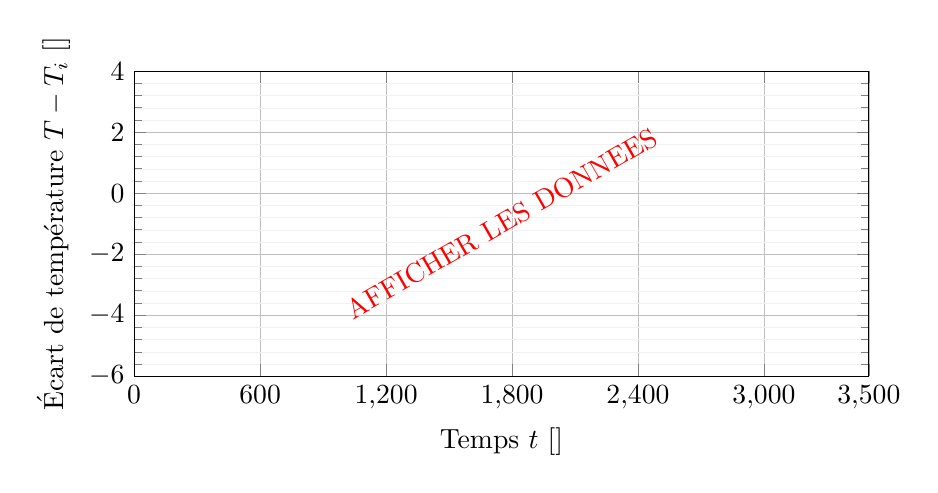
\begin{tikzpicture}
    \def\width{.9*\textwidth};
    \def\height{.5*\width};
    \def\legx{.5cm};
    \def\legy{\legx};
    
    \begin{axis}[name=plot,width={\width},height={\height},grid=both,minor tick num=4,
    grid style={line width=.1pt, draw=gray!10},
    major grid style={line width=.2pt,draw=gray!50},
    xlabel={Temps $t$ [\unit{\s}]},
    ylabel={\'Ecart de température $T-T_i$ [\unit{\degreeCelsius}]},
    xmin=0,xmax=3500,
	ymin=-6,ymax=4,
    xtick={0,600,1200,1800,2400,3000,3500},%ytick={0,9.1120/100000,1.4452/10000,2.5/10000,5/10000,1/1000},
    domain=0:100,
    legend style = {at={(1.01,1.05)},anchor = north east,cells={align=right}},legend columns=3,
    ]
    	
		
        
%        \legend{\\ \\};
    \end{axis}
    
    \draw (plot.center) node[rotate=30]{\color{red}AFFICHER LES DONNEES};
\end{tikzpicture}
    \caption{\'Evolution temporelle des températures dans la cavité d'adaptation d'impédance pour les expériences dans les orientation `\texttt{H1}' et `\texttt{H2}' à \textit{drive ratio} nul.}
    \label{fig:HeatOnly_CHXout_H1H2}
\end{figure}

\paragraph*{Avec acoustique}\label{chap:Acou_CHXout_H1H2_low}
Les premiers résultats sont obtenus pour les expériences horizontales `\texttt{H1}' et `\texttt{H2}' présentées sur les figures~\ref{fig:OrientationCore_H1} et \subref{fig:OrientationCore_H2}, à faible amplitude acoustique avec un \textit{drive ratio} $DR=\qty{.4}{\percent}$, et la température $\theta$ est tracée en fonction du temps $t$ sur la figure~\ref{fig:Acou_CHXout_H1H2_Low}. Pour les deux séries de mesures, c'est-à-dire les plans de thermocouples placés la verticale et l'horizontale et représentées respectivement en trait plein et trait tireté, la différence de température de \qty{2}{\degreeCelsius} entre le centre de l'échangeur froid et la source acoustique plus chaude apparaît après le démarrage de la pompe à chaleur à $t=\qty{100}{\second}$. Sur l'expérience réalisée dans l'orientation `\texttt{H2}', tous les thermocouples sont à la même altitude, et l'égalité des thermocouples~1~et~3 en bleu et en jaune permet notamment de visualiser une symétrie par rapport à un plan vertical passant par l'axe de symétrie du réfrigérateur. En revanche, cette symétrie n'est pas visible sur les courbes en traits pleins qui tracent les résultats de l'expérience menée en plaçant le réfrigérateur dans l'orientation `\texttt{H1}', puisqu'une dépendance de $\theta$ en fonction de $r$ est observable. En particulier, la courbe jaune correspondant au thermocouple~3 est la plus basse, en altitude comme en température, tandis que la courbe bleue qui représente le thermocouple~1 est la plus élevée des température mesurées sur l'échangeur froid, tout en y étant placée au plus haut. Toutefois, ce gradient de température n'est pas linéaire car la température au centre de l'échangeur froid mesurée par le thermocouple~2 n'est séparée que de \qty{.3}{\degreeCelsius} de la température mesurée par le thermocouple~3, tandis que cet écart est de \qty{2.5}{\degreeCelsius} avec le thermocouple~1. Cet dissymétrie est \textit{a priori} inattendue avec les résultats déjà obtenus dans les expériences sans acoustique.
\smallskip

%Tout d'abord, il est important de remarquer l'apparition de la différence de température après le démarrage du réfrigérateur entre la source acoustique principale (en noir) et le thermocouple 2 (en orange) situé en face, et ce, quel que soit l'orientation du plan de thermocouple. À cette différence de température s'ajoute la différence entre les courbes dans l'une et l'autre orientation, ce qui valide l'hypothèse de l'influence de la direction de la gravité sur la distribution de température dans la cavité d'adaptation d'impédance proposée par l'étude du nombre de Rayleigh. Notamment, la courbe jaune, qui représente la température mesurée par le thermocouple~3, atteint la température la plus faible quand ce capteur se trouve à la position la plus basse (courbe en trait plein), alors que lorsqu'il est à la même altitude que les autres thermocouples (courbe en trait tireté), il est également à la même température que le thermocouple~1. Un plan de symétrie vertical semble donc être présent lorsque le réfrigérateur est en position horizontale, ce qui est visible dans les expériences où les thermocouples sont sur un plan horizontal. En revanche, en vertical on s'attend à avoir un gradient linéaire mais en fait bof (comparer avec résultats lisn)

\begin{figure}[!ht]
    \centering
    \external{fig_Acou_CHXout_H1H2_Low}
%    \externalremake
    \begin{tikzpicture}
    \def\width{.9*\textwidth};
    \def\height{.5*\width};
    \def\legx{.5cm};
    \def\legy{\legx};
    
    \begin{axis}[width={\width},height={\height},grid=both,minor tick num=4,
    grid style={line width=.1pt, draw=gray!10},
    major grid style={line width=.2pt,draw=gray!50},
    xlabel={Temps $t$ [\unit{\s}]},
    ylabel={\'Ecart de température $\theta$ [\unit{\degreeCelsius}]},
    xmin=0,xmax=3500,
	ymin=-3,ymax=2,
    xtick={0,600,1200,1800,2400,3000,3500},%ytick={},
    domain=0:100,
    legend style = {at={(1.01,1.05)},anchor = north east,cells={align=right},rounded corners},legend columns=3,
%    legend cell align=right
    ]
    
		\addlegendimage{legend image with text=}
		\addlegendentry{}
		\addlegendimage{legend image with text=`\texttt{H1}'}
		\addlegendentry{}
		\addlegendimage{legend image with text=`\texttt{H2}'} 
		\addlegendentry{}   
    
    	\addlegendimage{legend image with text=TC 0}
    	\addlegendentry{}
    	
    	\addplot[ultra thick,black] file {{../fig/fig_ConvNat_Acou/data/DataMatTxtH1H2Low/data_TC0_0beg_RixLow_PhaseRIXHP-60°_OrientationH1_Qc0W_Serie1.txt}};\addlegendentry{}%\addlegendentry{TC src. ac. 1 (H1)}
		\addplot[ultra thick,black,dashed] file {{../fig/fig_ConvNat_Acou/data/DataMatTxtH1H2Low/data_TC0_0beg_RixLow_PhaseRIXHP-60°_OrientationH2_Qc0W_Serie1.txt}};\addlegendentry{}%\addlegendentry{TC src. ac. 1 (H2)}
		
		\addlegendimage{legend image with text=TC 1}
		\addlegendentry{}
		
    	\addplot[ultra thick,MatlabBlue] file {{../fig/fig_ConvNat_Acou/data/DataMatTxtH1H2Low/data_TC1_0beg_RixLow_PhaseRIXHP-60°_OrientationH1_Qc0W_Serie1.txt}};\addlegendentry{}
    	\addplot[ultra thick,MatlabBlue,dashed] file {{../fig/fig_ConvNat_Acou/data/DataMatTxtH1H2Low/data_TC1_0beg_RixLow_PhaseRIXHP-60°_OrientationH2_Qc0W_Serie1.txt}};\addlegendentry{}
    	
		\addlegendimage{legend image with text=TC 2}
		\addlegendentry{}   	
    	
    	\addplot[ultra thick,MatlabOrange] file {{../fig/fig_ConvNat_Acou/data/DataMatTxtH1H2Low/data_TC2_0beg_RixLow_PhaseRIXHP-60°_OrientationH1_Qc0W_Serie1.txt}};\addlegendentry{}
    	\addplot[ultra thick,MatlabOrange,dashed] file {{../fig/fig_ConvNat_Acou/data/DataMatTxtH1H2Low/data_TC2_0beg_RixLow_PhaseRIXHP-60°_OrientationH2_Qc0W_Serie1.txt}};\addlegendentry{}
    	
    	\addlegendimage{legend image with text=TC 3}
    	\addlegendentry{}
    	
    	\addplot[ultra thick,MatlabYellow] file {{../fig/fig_ConvNat_Acou/data/DataMatTxtH1H2Low/data_TC3_0beg_RixLow_PhaseRIXHP-60°_OrientationH1_Qc0W_Serie1.txt}};\addlegendentry{}    	
    	\addplot[ultra thick,MatlabYellow,dashed] file {{../fig/fig_ConvNat_Acou/data/DataMatTxtH1H2Low/data_TC3_0beg_RixLow_PhaseRIXHP-60°_OrientationH2_Qc0W_Serie1.txt}};\addlegendentry{}
        
%        \legend{\\ \\};
    \end{axis}
\end{tikzpicture}
    \caption{\'Evolution temporelle des températures dans la cavité d'adaptation d'impédance pour les expériences dans les orientations `\texttt{H1}' et `\texttt{H2}' à faible \textit{drive ratio} $DR=\qty{.4}{\percent}$.}
    \label{fig:Acou_CHXout_H1H2_Low}
\end{figure}

La figure~\ref{fig:Acou_CHXout_H1H2_Mid} représente également l'évolution temporelle de la température $\theta$ dans la cavité, pour l'amplitude acoustique dite \og moyenne \fg{}  de \textit{drive ratio} $DR=\qty{2}{\percent}$. Après l'apparition de l'écart de température échangeur froid - source acoustique, qui vaut \qty{10.2}{\degreeCelsius} en `\texttt{H1}' et \qty{15.2}{\degreeCelsius} en `\texttt{H2}', des symptômes similaires à l'expérience à faible amplitude sont observables. À nouveau, les thermocouples~1~et~3 affichent des températures égales quand leurs altitudes sont égales (orientation `\texttt{H2}') et la symétrie des températures par rapport au plan vertical qui passe par le centre du noyau thermoacoustique est à nouveau mise en évidence. En revanche,  un écart de \qty{10}{\degreeCelsius} est visible lorsqu'ils sont l'un au dessus de l'autre (orientation `\texttt{H1}'). Dans cette orientation, le gradient vertical de température n'est toujours pas linéaire, puisque les températures~2~et~3 sont égales l'une à l'autre, \qty{10.2}{\degreeCelsius} en deça de la température mesurée par le thermocouple~1. 
\smallskip 

\begin{figure}[!ht]
    \centering
    \external{fig_Acou_CHXout_H1H2_Mid}
%    \externalremake
    \input{../fig/fig_ConvNat_Acou/tex/fig_Acou_CHXout_H1H2_Mid}
    \caption{\'Evolution temporelle des températures dans la cavité d'adaptation d'impédance pour les expériences dans les orientations `\texttt{H1}' et `\texttt{H2}' à \textit{drive ratio} intermédiaire $DR~=~\qty{2}{\percent}$.}
    \label{fig:Acou_CHXout_H1H2_Mid}
\end{figure}

L'évolution de température $\theta$ au cours de l'expérience à l'amplitude acoustique \og élevée \fg{} est représentée sur la figure~\ref{fig:Acou_CHXout_H1H2_High}. Dans cette expérience, le \textit{drive ratio} est $DR=\qty{3.5}{\percent}$, ce qui correspond à l'amplitude pour laquelle les meilleures performances avaient été obtenues pour cette machine dotée du précédent noyau thermoacoustique. Les résultats de cette expérience sont assez similaire à ceux obtenus pour les faible et moyenne amplitude, à quelques différences près. Après l'établissement de la différence de température de \qty{16}{\degreeCelsius} entre le centre de l'échangeur froid et la source acoustique principale suite au démarrage de la machine, plusieurs effets sont à noter. Premièrement, la distribution de température est bien différente entre le cas `\texttt{H1}' où le plan de thermocouples est vertical et le cas `\texttt{H2}' où il est horizontal. En particulier, les courbes noires d'une part et les courbes rouges d'autre part se superposent d'une orientation à l'autre, ce qui est un effet attendu au vu de leur position sur l'axe de symétrie du réfrigérateur. Ensuite, la température le long de la dimension verticale $\mathbf e_r^{//\mathbf g}$ augmente avec cette dernière, encore une fois avec les thermocouples~2~et~3 à \qty{2}{\degreeCelsius} l'un de l'autre, et le thermocouple~1 \qty{12}{\degreeCelsius} au-dessus. Contrairement aux observations précédentes de ce gradient, à cette amplitude c'est le thermocouple~2 qui indique la température la plus basse, bien qu'il se trouve \qty{74}{\milli\meter} au-dessus du thermocouple~3. Cela dit, cet écart entre les deux thermocouples~2~et~3 est faible devant la valeur de température atteinte lors du fonctionnement de la machine et du refroidissement de cette zone, c'est-à-dire \qty{-23}{\degreeCelsius}. Il est possible de considérer cet écart comme une incertitude de mesure et ainsi se ramener à une analyse équivalente à celles des amplitudes plus faibles. Dans l'orientation `\texttt{H2}', la symétrie par rapport au plan vertical qui était visible aux amplitudes faibles et moyennes ne l'est plus. Les thermocouples~1~et~3 ne sont plus égaux, et sont séparés de \qty{2}{\degreeCelsius}. Cependant, pour les mêmes raisons que précédemment, l'écart est à nouveau considéré comme négligeable devant la valeur de la température atteinte, et les mêmes analyses qu'aux amplitudes faible et moyenne sont proposées.

\begin{figure}[!ht]
    \centering
    \external{fig_Acou_CHXout_H1H2_High}
%    \externalremake
    \input{../fig/fig_ConvNat_Acou/tex/fig_Acou_CHXout_H1H2_High}
    \caption{\'Evolution temporelle des températures dans la cavité d'adaptation d'impédance pour les expériences dans les orientations `\texttt{H1}' et `\texttt{H2}' à haut \textit{drive ratio} $DR=\qty{3.4}{\percent}$.}
    \label{fig:Acou_CHXout_H1H2_High}
\end{figure}


\subsubsection{Réfrigérateur vertical}
\paragraph*{Sans acoustique}
\echaf{ICI les manips heat only}

\begin{figure}[!ht]
    \centering
    \external{fig_HeatOnly_CHXout_V1V2}
%    \externalremake
    \begin{tikzpicture}
    \def\width{.9*\textwidth};
    \def\height{.5*\width};
    \def\legx{.5cm};
    \def\legy{\legx};
    
    \begin{axis}[name=plot,width={\width},height={\height},grid=both,minor tick num=4,
    grid style={line width=.1pt, draw=gray!10},
    major grid style={line width=.2pt,draw=gray!50},
    xlabel={Temps $t$ [\unit{\s}]},
    ylabel={\'Ecart de température $T-T_i$ [\unit{\degreeCelsius}]},
    xmin=0,xmax=3500,
	ymin=-5,ymax=80,
    xtick={0,600,...,3000,3500},
    ytick={-5,0,10,...,80},
    domain=0:100,
    legend style = {at={(.01,1.05)},anchor = north west,cells={align=right},rounded corners},legend columns=3, fill opacity=1, text opacity=1
    ]
    	
    	
    	\addlegendimage{legend image with text=}
		\addlegendentry{}
		\addlegendimage{legend image with text={`\texttt{V1}'}}
		\addlegendentry{}
		\addlegendimage{legend image with text=`\texttt{V2}'} 
		\addlegendentry{}   
    
    	\addlegendimage{legend image with text=TC 0}
    	\addlegendentry{}
    	
    	\addplot[ultra thick,black] file {{../fig/fig_ConvNat_HeatOnly/data/FixedPower/V1V2/data_TC0_0beg_RixOff_PhaseRIXHP-60°_OrientationV1_Qc40W_Serie3.txt}};\addlegendentry{}
		\addplot[ultra thick,black,dashed] file {{../fig/fig_ConvNat_HeatOnly/data/FixedPower/V1V2/data_TC0_0beg_RixOff_PhaseRIXHP-60°_OrientationV2_Qc40W_Serie1.txt}};\addlegendentry{}
		
		\addlegendimage{legend image with text=TC 1}
		\addlegendentry{}
		
    	\addplot[ultra thick,MatlabBlue] file {{../fig/fig_ConvNat_HeatOnly/data/FixedPower/V1V2/data_TC1_0beg_RixOff_PhaseRIXHP-60°_OrientationV1_Qc40W_Serie3.txt}};\addlegendentry{}
    	\addplot[ultra thick,MatlabBlue,dashed] file {{../fig/fig_ConvNat_HeatOnly/data/FixedPower/V1V2/data_TC1_0beg_RixOff_PhaseRIXHP-60°_OrientationV2_Qc40W_Serie1.txt}};\addlegendentry{}
    	
    	\addlegendimage{legend image with text=TC 2}
		\addlegendentry{}
		
    	\addplot[ultra thick,MatlabOrange] file {{../fig/fig_ConvNat_HeatOnly/data/FixedPower/V1V2/data_TC2_0beg_RixOff_PhaseRIXHP-60°_OrientationV1_Qc40W_Serie3.txt}};\addlegendentry{}
    	\addplot[ultra thick,MatlabOrange,dashed] file {{../fig/fig_ConvNat_HeatOnly/data/FixedPower/V1V2/data_TC2_0beg_RixOff_PhaseRIXHP-60°_OrientationV2_Qc40W_Serie1.txt}};\addlegendentry{}
    	
		\addlegendimage{legend image with text=TC 3}
		\addlegendentry{}
		
    	\addplot[ultra thick,MatlabYellow] file {{../fig/fig_ConvNat_HeatOnly/data/FixedPower/V1V2/data_TC3_0beg_RixOff_PhaseRIXHP-60°_OrientationV1_Qc40W_Serie3.txt}};\addlegendentry{}    	
    	\addplot[ultra thick,MatlabYellow,dashed] file {{../fig/fig_ConvNat_HeatOnly/data/FixedPower/V1V2/data_TC3_0beg_RixOff_PhaseRIXHP-60°_OrientationV2_Qc40W_Serie1.txt}};\addlegendentry{}
		
        
%        \legend{\\ \\};
    \end{axis}
%    \draw (plot.center) node[rotate=30]{\color{red}AFFICHER LES DONNEES};
\end{tikzpicture}
    \caption{\'Evolution temporelle des températures dans la cavité d'adaptation d'impédance pour les expériences dans les orientations `\texttt{V1}' et `\texttt{V2}' à \textit{drive ratio} nul.}
    \label{fig:HeatOnly_CHXout_V1V2}
\end{figure}

\paragraph*{Avec acoustique}
La figure~\ref{fig:Acou_CHXout_V1V2_Low} trace les températures mesurées dans la cavité d'adaptation d'impédance pour des expériences où le réfrigérateur est placé dans les orientations verticales présentées figures~\ref{fig:OrientationCore_V1} et \subref{fig:OrientationCore_V2}, pour une amplitude \og faible \fg{} soit un \textit{drive ratio} $DR=\qty{.4}{\percent}$. Contrairement aux expériences horizontales où les effets de convection naturelle sont toujours présents mais pas toujours visibles, dans les expériences verticales il existe une configuration favorable à la mise en place d'une instabilité de convection naturelle de type Rayleigh-Bénard, et l'autre, inverse, qui est stable. La première configuration est l'orientation `\texttt{V1}', car la source acoustique y est en dessous du noyau thermoacoustique, car le sens du gradient de température est opposé à la gravité, tandis que la seconde est l'orientation `\texttt{V2}' où la source acoustique est au-dessus du noyau. Dans cette dernière orientation, le gradient de température est dans le même sens que la gravité, et il n'y a pas de flux de chaleur qui apparaît de manière spontanée. La première remarque concerne la différence d'aspect de l'évolution des températures entre une orientation et l'autre, malgré une axi-symétrie visible dans les deux cas et attendue au vu de la colinéarité de la dimensions axiale $\mathbf e_x$ et de la gravité $\mathbf g$. En observant les tracés en lignes tiretées, qui tracent l'évolution de la température $\theta$ au cours de l'expérience dans l'orientation `\texttt{V2}', une différence de température de \qty{3.2}{\degreeCelsius} entre l'échangeur froid du noyau et la source acoustique principale plus chaude apparaît et se maintient durant toute la durée de l'expérience. C'est d'ailleurs le plus grand écart de température relevé dans cette zone. Plus précisément, la température mesurée devant la source acoustique principale baisse \qty{.8}{\degreeCelsius} même après démarrage de celle-ci, ce qui est assez faible pour être en accord avec l'hypothèse de stabilité des températures en l'absence de flux massique causé par la convection naturelle. Dans l'orientation inverse `\texttt{V1}' représentée par les tracés en traits pleins, la différence de température apparaît également après le démarrage des sources acoustiques. Toutefois, après \qty{1800}{\second} les thermocouples sur l'axe de symétrie et en vis à vis l'un de l'autre, autrement dit devant la source acoustique principale et le thermocouple~2, affichent la même température. De manière plus générale, tous les thermocouple de cette zone d'adaptation d'impédance sont à des températures plus homogènes, puisque l'écart maximum de températures est dans ce cas de \qty{.8}{\degreeCelsius}. Un effet très remarquable pour cette orientation est l'évolution de température en deux étapes : la première, pendant laquelle la température sur l'échangeur froid diminue et qui s'étend du démarrage des sources à \qty{1100}{\second}, et la seconde, de cet instant jusqu'à la fin de l'acquisition et où un réchauffement des thermocouples sur l'échangeur froid apparaît. Il semblerait qu'il s'agisse là de la manifestations de deux effets aux constantes de temps différentes, l'effet thermoacoustique qui agit dès l'allumage des sources acoustiques et la convection naturelle, plus lente. Il est supposé que lors de la première étape, la différence de température augmente peu à peu et le nombre de Rayleigh avec elle, et ce, jusqu'au dépassement de la valeur critique de $\Rayleigh_c$. Au delà de cette valeur \echaf{que l'on peut estimer expérimentalement avec l'équation~\eqref{eq:NbrRayleigh} appliquée à la différence de température $\Delta \theta|_{t=\qty{1100}{\second}}$ ou bien quand $\partial^2_{tt}\theta=\num{0}$}, une cellule de convection de type Rayleigh-Bénard se met en place, et déplace avec le fluide en mouvement une certaine quantité de chaleur $Q_{\sf conv}$ de la source acoustique vers l'échangeur froid. Le gradient de température entre la source acoustique principale et l'échangeur froid n'étant pas fixé, les deux extrémités de la cavité d'adaptation d'impédance voient leur température converger vers un point d'équilibre, à la valeur moyenne des températures mesurées au mêmes emplacements dans l'orientation `\texttt{V2}'.
\smallskip
 
\begin{figure}[!ht]
    \centering
    \external{fig_Acou_CHXout_V1V2_Low}
%    \externalremake
    \begin{tikzpicture}
    \def\width{.9*\textwidth};
    \def\height{.5*\width};
    \def\legx{.5cm};
    \def\legy{\legx};
    
    \begin{axis}[width={\width},height={\height},grid=both,minor tick num=4,
    grid style={line width=.1pt, draw=gray!10},
    major grid style={line width=.2pt,draw=gray!50},
    xlabel={Temps $t$ [\unit{\s}]},
    ylabel={\'Ecart de température $\tau$ [\unit{\degreeCelsius}]},
    xmin=0,xmax=3500,
	 ymin=-5,ymax=4,
    xtick={0,600,1200,1800,2400,3000,3500},%ytick={0,9.1120/100000,1.4452/10000,2.5/10000,5/10000,1/1000},
    domain=0:100,
    legend style = {at={(1.01,1.05)},anchor = north east},legend columns=3,
%    legend cell align={right},
    ]
%		\addplot[very thick,black] file {{../fig/fig_ConvNat_Acou/data/DataMatTxtV1V2Low/data_TC0_0beg_RixLow_PhaseRIXHP-60°_OrientationV1_Qc0W_Serie1.txt}};\addlegendentry{TC src. ac. 1 (V1)}
%		\addplot[very thick,black!50] file {{../fig/fig_ConvNat_Acou/data/DataMatTxtV1V2Low/data_TC0_0beg_RixLow_PhaseRIXHP-60°_OrientationV2_Qc0W_Serie1.txt}};\addlegendentry{TC src. ac. 1 (V2)}
%    	\addplot[very thick,Blue1] file {{../fig/fig_ConvNat_Acou/data/DataMatTxtV1V2Low/data_TC1_0beg_RixLow_PhaseRIXHP-60°_OrientationV1_Qc0W_Serie1.txt}};\addlegendentry{TC 1}
%    	\addplot[very thick,Blue4] file {{../fig/fig_ConvNat_Acou/data/DataMatTxtV1V2Low/data_TC1_0beg_RixLow_PhaseRIXHP-60°_OrientationV2_Qc0W_Serie1.txt}};\addlegendentry{TC 1}
%    	\addplot[very thick,Blue2] file {{../fig/fig_ConvNat_Acou/data/DataMatTxtV1V2Low/data_TC2_0beg_RixLow_PhaseRIXHP-60°_OrientationV1_Qc0W_Serie1.txt}};\addlegendentry{TC 2}
%    	\addplot[very thick,Blue5] file {{../fig/fig_ConvNat_Acou/data/DataMatTxtV1V2Low/data_TC2_0beg_RixLow_PhaseRIXHP-60°_OrientationV2_Qc0W_Serie1.txt}};\addlegendentry{TC 2}
%    	\addplot[very thick,Blue3] file {{../fig/fig_ConvNat_Acou/data/DataMatTxtV1V2Low/data_TC3_0beg_RixLow_PhaseRIXHP-60°_OrientationV1_Qc0W_Serie1.txt}};\addlegendentry{TC 3}    	
%    	\addplot[very thick,Blue6] file {{../fig/fig_ConvNat_Acou/data/DataMatTxtV1V2Low/data_TC3_0beg_RixLow_PhaseRIXHP-60°_OrientationV2_Qc0W_Serie1.txt}};\addlegendentry{TC 3}
    	
		\addlegendimage{legend image with text=}
		\addlegendentry{}
		\addlegendimage{legend image with text=V1}
		\addlegendentry{}
		\addlegendimage{legend image with text=V2} 
		\addlegendentry{}       	
    	
    	\addlegendimage{legend image with text=Source acoustique principale}
    	\addlegendentry{}
    	
    	\addplot[ultra thick,black] file {{../fig/fig_ConvNat_Acou/data/DataMatTxtV1V2Low/data_TC0_0beg_RixLow_PhaseRIXHP-60°_OrientationV1_Qc0W_Serie1.txt}};\addlegendentry{}
		\addplot[ultra thick,black,dashed] file {{../fig/fig_ConvNat_Acou/data/DataMatTxtV1V2Low/data_TC0_0beg_RixLow_PhaseRIXHP-60°_OrientationV2_Qc0W_Serie1.txt}};\addlegendentry{}
		
		\addlegendimage{legend image with text=TC 1}
		\addlegendentry{}
		
    	\addplot[ultra thick,MatlabBlue] file {{../fig/fig_ConvNat_Acou/data/DataMatTxtV1V2Low/data_TC1_0beg_RixLow_PhaseRIXHP-60°_OrientationV1_Qc0W_Serie1.txt}};\addlegendentry{}
    	\addplot[ultra thick,MatlabBlue,dashed] file {{../fig/fig_ConvNat_Acou/data/DataMatTxtV1V2Low/data_TC1_0beg_RixLow_PhaseRIXHP-60°_OrientationV2_Qc0W_Serie1.txt}};\addlegendentry{}
    	
    	\addlegendimage{legend image with text=TC 2}
		\addlegendentry{}
		
    	\addplot[ultra thick,MatlabOrange] file {{../fig/fig_ConvNat_Acou/data/DataMatTxtV1V2Low/data_TC2_0beg_RixLow_PhaseRIXHP-60°_OrientationV1_Qc0W_Serie1.txt}};\addlegendentry{}
    	\addplot[ultra thick,MatlabOrange,dashed] file {{../fig/fig_ConvNat_Acou/data/DataMatTxtV1V2Low/data_TC2_0beg_RixLow_PhaseRIXHP-60°_OrientationV2_Qc0W_Serie1.txt}};\addlegendentry{}
    	
    	\addlegendimage{legend image with text=TC 3}
		\addlegendentry{}
		
    	\addplot[ultra thick,MatlabYellow] file {{../fig/fig_ConvNat_Acou/data/DataMatTxtV1V2Low/data_TC3_0beg_RixLow_PhaseRIXHP-60°_OrientationV1_Qc0W_Serie1.txt}};\addlegendentry{}    	
    	\addplot[ultra thick,MatlabYellow,dashed] file {{../fig/fig_ConvNat_Acou/data/DataMatTxtV1V2Low/data_TC3_0beg_RixLow_PhaseRIXHP-60°_OrientationV2_Qc0W_Serie1.txt}};\addlegendentry{}
        
%        \legend{\\ \\};
    \end{axis}
\end{tikzpicture}
    \caption{\'Evolution temporelle des températures dans la cavité d'adaptation d'impédance pour les expériences dans les orientations `\texttt{V1}' et `\texttt{V2}' à faible \textit{drive ratio} $DR=\qty{.4}{\percent}$.}
    \label{fig:Acou_CHXout_V1V2_Low}
\end{figure}

À moyenne amplitude pour un \textit{drive ratio} $DR=\qty{2}{\percent}$, les résultats des expériences sont tracés sur la figure~\ref{fig:Acou_CHXout_V1V2_Mid}. Pour cette série, il est difficile de conclure sur le comportement d'une supposée cellule de convection naturelle : les différences entre les deux configurations ne correspondent pas aux tendances mises en évidence par les expériences à faible amplitude.
\smallskip

\begin{figure}[!ht]
    \centering
    \external{fig_Acou_CHXout_V1V2_Mid}
%    \externalremake
    \input{../fig/fig_ConvNat_Acou/tex/fig_Acou_CHXout_V1V2_Mid}
    \caption{\'Evolution temporelle des températures dans la cavité d'adaptation d'impédance pour les expériences dans les orientations `\texttt{V1}' et `\texttt{V2}' à \textit{drive ratio} intermédiaire $DR~=~\qty{2}{\percent}$.}
    \label{fig:Acou_CHXout_V1V2_Mid}
\end{figure}

En revanche, la figure~\ref{fig:Acou_CHXout_V1V2_High} qui présente les résultats obtenus à haute amplitude, c'est-à-dire pour un \textit{drive ratio} de $DR=\qty{3.5}{\percent}$, les effets liés à la convection naturelle sont visibles. En effet, les tendances sont les mêmes qu'à faible amplitude acoustique, à d'autres échelles en termes d'amplitude ce température ou de temps, et une différence de résultats de l'ordre de \qty{6}{\degreeCelsius} est manifeste en fonction de l'orientation du réfrigérateur. Notamment, les courbes en trait tiretés qui représentent l'orientation `\texttt{V2}' montrent à nouveau un refroidissement de la zone avant une stabilisation des températures, tandis que les courbes en trait plein affichent un réchauffement à $t=\qty{400}{\second}$ entre le refroidissement initial et la stabilisation des températures dans la cavité conique dans l'orientation `\texttt{V1}'.

\begin{figure}[!ht]
    \centering
    \external{fig_Acou_CHXout_V1V2_High}
%    \externalremake
    \input{../fig/fig_ConvNat_Acou/tex/fig_Acou_CHXout_V1V2_High}
    \caption{\'Evolution temporelle des températures dans la cavité d'adaptation d'impédance pour les expériences dans les orientations `\texttt{V1}' et `\texttt{V2}' à haut \textit{drive ratio} $DR=\qty{3.5}{\percent}$.}
    \label{fig:Acou_CHXout_V1V2_High}
\end{figure}



\subsection{À l'intérieur du régénérateur}
\subsubsection{Réfrigérateur horizontal}
\paragraph*{Amplitude acoustique nulle}

\begin{figure}[!ht]
    \centering
	\begin{subfigure}{\textwidth}
		\centering
		\external{fig_HeatOnly_CHXin_H1H2}
%		\externalremake
		\input{../fig/fig_ConvNat_HeatOnly/tex/fig_HeatOnly_CHXin_H1H2}
		\caption{\numlist{4;5;6}}
		\label{fig:HeatOnly_CHXin_H1H2}
	\end{subfigure}	\vspace{1em}
	
	\begin{subfigure}{\textwidth}
		\centering
		\external{fig_HeatOnly_Regmid_H1H2}
%		\externalremake
		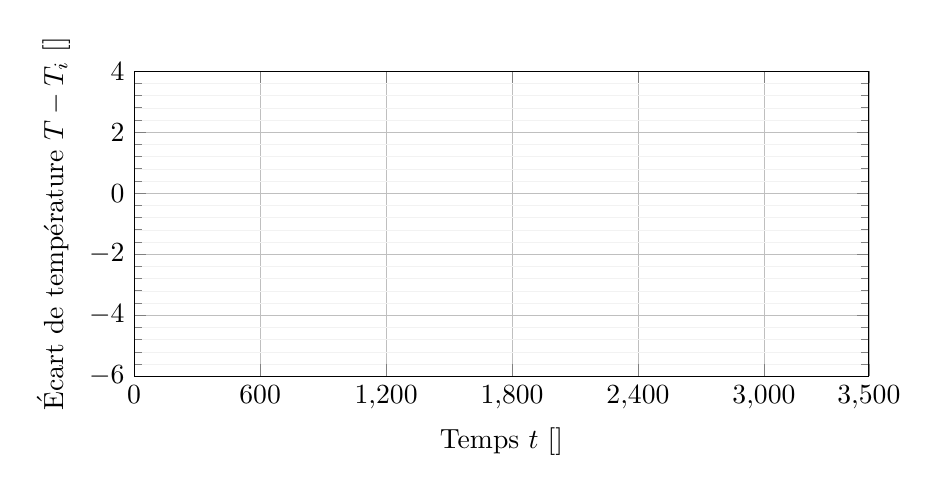
\begin{tikzpicture}
    \def\width{.9*\textwidth};
    \def\height{.5*\width};
    \def\legx{.5cm};
    \def\legy{\legx};
    
    \begin{axis}[width={\width},height={\height},grid=both,minor tick num=4,
    grid style={line width=.1pt, draw=gray!10},
    major grid style={line width=.2pt,draw=gray!50},
    xlabel={Temps $t$ [\unit{\s}]},
    ylabel={\'Ecart de température $T-T_i$ [\unit{\degreeCelsius}]},
    xmin=0,xmax=3500,
	ymin=-6,ymax=4,
    xtick={0,600,1200,1800,2400,3000,3500},%ytick={0,9.1120/100000,1.4452/10000,2.5/10000,5/10000,1/1000},
    domain=0:100,
    legend style = {at={(.95,.05)},anchor = south east},legend columns=2
    ]
    	
		
        
%        \legend{\\ \\};
    \end{axis}
\end{tikzpicture}
		\caption{\numlist{7;8;9}}
		\label{fig:HeatOnly_Regmid_H1H2}
	\end{subfigure}	\vspace{1em} 
	
	\begin{subfigure}{\textwidth}
		\centering
		\external{fig_HeatOnly_AHXin_H1H2}
%		\externalremake
		\input{../fig/fig_ConvNat_HeatOnly/tex/fig_HeatOnly_AHXin_H1H2}
		\caption{\numlist{10;11;12}}
		\label{fig:HeatOnly_AHXin_H1H2}
	\end{subfigure}		   
    \caption{\echaf{changer caption}}
    \label{fig:HeatOnly_H1H2}
\end{figure}


\paragraph*{Faible amplitude acoustique}
Les figures~\ref{fig:Acou_CHXin_H1H2_Low} à \ref{fig:Acou_AHXin_H1H2_Low} montrent les résultats à faible amplitude acoustique, pour les trois positions axiales le long du régénérateur. Dans cette configuration, le nombre de Rayleigh $\Rayleigh_p$ est de \echaf{Valeur}. 

Tout d'abord, du côté de l'échangeur froid dont les résultats d'expériences sont affichés sur la figure~\ref{fig:Acou_CHXin_H1H2_Low}, une tendance similaire à ce qui a été montré dans la cavité d'adaptation d'impédance sur la figure~\ref{fig:Acou_CHXout_H1H2_Low} est visible. Notamment, la température mesurée par le thermocouple~5 placé au centre du régénérateur est la même dans les deux orientations, avec une diminution de \qty{5.2}{\degreeCelsius} par rapport à la température initiale pour l'orientation `\texttt{H1}', et de \qty{4.8}{\degreeCelsius} pour l'orientation `\texttt{H2}'. La périphérie du régénérateur, dont les températures sont acquises par les thermocouples~4~et~6, voient à l'inverse leur température varier en fonction de l'orientation. Dans l'orientation `\texttt{H1}', les températures données par les thermocouples~5~et~6 sont respectivement égales à \qty{-5.2}{\degreeCelsius} et \qty{-4.8}{\degreeCelsius}, et le thermocouple~4 indique une température de \qty{-2.9}{\degreeCelsius}. En revanche, dans l'orientation `\texttt{H2}' ce sont cette fois les thermocouples~4~et~6 qui sont proches car égaux à \qty{-3}{\degreeCelsius} et \qty{-3.2}{\degreeCelsius}, et le thermocouple~5 qui relève \qty{-4.8}{\degreeCelsius}. La symétrie par rapport au plan vertical passant par le centre du régénérateur est ainsi maintenue du côté froid intérieur du régénérateur, de même que ce que l'étude dans la cavité d'adapatation d'impédance montre le paragraphe~§\ref{chap:Acou_CHXout_H1H2_low}.

\begin{figure}[!ht]
    \centering
	\begin{subfigure}{\textwidth}
		\centering
		\external{fig_Acou_CHXin_H1H2_Low}
%    	\externalremake
        \input{../fig/fig_ConvNat_Acou/tex/fig_Acou_CHXin_H1H2_Low}
		\caption{}
		\label{fig:Acou_CHXin_H1H2_Low}
	\end{subfigure} \vspace{1em}
	
	\begin{subfigure}{\textwidth}
		\centering
		\external{fig_Acou_Regmid_H1H2_Low}
%    	\externalremake
        \begin{tikzpicture}
    \def\width{.9*\textwidth};
    \def\height{.25*\textheight};
    \def\legx{.5cm};
    \def\legy{\legx};
    
    \begin{axis}[name=boundary,width={\width},height={\height},grid=both,minor tick num=4,
    grid style={line width=.1pt, draw=gray!10},
    major grid style={line width=.2pt,draw=gray!50},
    xlabel={Temps $t$ [\unit{\s}]},
    ylabel={\'Ecart de température $\tau$ [\unit{\degreeCelsius}]},
    xmin=0,xmax=3500,
	ymin=-6,ymax=4,
    xtick={0,600,1200,1800,2400,3000,3500},%ytick={0,9.1120/100000,1.4452/10000,2.5/10000,5/10000,1/1000},
    domain=0:100,
    legend style = {at={(1.01,.05)},anchor = south east,rounded corners},legend columns=3,
    ]
    
    \addlegendimage{legend image with text=}
		\addlegendentry{}
		\addlegendimage{legend image with text=`\texttt{H1}'}
		\addlegendentry{}
		\addlegendimage{legend image with text=`\texttt{H2}'} 
		\addlegendentry{}       	
    	
    	\addlegendimage{legend image with text=TC 7}
    	\addlegendentry{}
    	
		\addplot[ultra thick,MatlabBlue] file {{../fig/fig_ConvNat_Acou/data/DataMatTxtH1H2Low/data_TC7_0beg_RixLow_PhaseRIXHP-60°_OrientationH1_Qc0W_Serie1.txt}};\addlegendentry{}
    	\addplot[ultra thick,MatlabBlue,dashed] file {{../fig/fig_ConvNat_Acou/data/DataMatTxtH1H2Low/data_TC7_0beg_RixLow_PhaseRIXHP-60°_OrientationH2_Qc0W_Serie1.txt}};\addlegendentry{}
    	
    	\addlegendimage{legend image with text=TC 8}
    	\addlegendentry{}
    	 
    	\addplot[ultra thick,MatlabOrange] file {{../fig/fig_ConvNat_Acou/data/DataMatTxtH1H2Low/data_TC8_0beg_RixLow_PhaseRIXHP-60°_OrientationH1_Qc0W_Serie1.txt}};\addlegendentry{}
    	\addplot[ultra thick,MatlabOrange,dashed] file {{../fig/fig_ConvNat_Acou/data/DataMatTxtH1H2Low/data_TC8_0beg_RixLow_PhaseRIXHP-60°_OrientationH2_Qc0W_Serie1.txt}};\addlegendentry{}
    	
    	\addlegendimage{legend image with text=TC 9}
    	\addlegendentry{}
    	
    	\addplot[ultra thick,MatlabYellow] file {{../fig/fig_ConvNat_Acou/data/DataMatTxtH1H2Low/data_TC9_0beg_RixLow_PhaseRIXHP-60°_OrientationH1_Qc0W_Serie1.txt}};\addlegendentry{}
    	\addplot[ultra thick,MatlabYellow,dashed] file {{../fig/fig_ConvNat_Acou/data/DataMatTxtH1H2Low/data_TC9_0beg_RixLow_PhaseRIXHP-60°_OrientationH2_Qc0W_Serie1.txt}};\addlegendentry{}
    	
%        \legend{\\ \\};
    \end{axis}
\end{tikzpicture}
		\caption{}
		\label{fig:Acou_Regmid_H1H2_Low}
	\end{subfigure} \vspace{1em}
	
	\begin{subfigure}{\textwidth}
		\centering
		\external{fig_Acou_AHXin_H1H2_Low}
%    	\externalremake
        \input{../fig/fig_ConvNat_Acou/tex/fig_Acou_AHXin_H1H2_Low}
		\caption{}
		\label{fig:Acou_AHXin_H1H2_Low}
	\end{subfigure}	
    \caption{\'Evolution temporelle des températures dans le régénérateur pour les expériences dans les orientations `\texttt{H1}' et `\texttt{H2}' à faible \textit{drive ratio} $DR=\qty{.4}{\percent}$. \subref{fig:Acou_CHXin_H1H2_Low} côté froid (TC \numlist{4;5;6}), \subref{fig:Acou_Regmid_H1H2_Low} milieu (TC \numlist{7;8;9}), \subref{fig:Acou_AHXin_H1H2_Low} côté ambiant (TC \numlist{10;11;12}).} 
    \label{fig:Acou_H1H2_Low}
\end{figure}

%\begin{figure}[!ht]
%    \centering
%    \external{fig_Acou_CHXin_H1H2_Low}
%%    \externalremake
%    \input{../fig/fig_ConvNat_Acou/tex/fig_Acou_CHXin_H1H2_Low}
%    \caption{\'Evolution temporelle des températures au côté froid du régénérateur pour les expériences dans les orientations `\texttt{H1}' et `\texttt{H2}' à faible \textit{drive ratio} $DR=\qty{.4}{\percent}$.}
%    \label{fig:Acou_CHXin_H1H2_Low}
%\end{figure}

La figure~\ref{fig:Acou_Regmid_H1H2_Low} présente la distribution de température au milieu du régénérateur. Dans ce graphique, il est possible de voir que même à partir du moment où les sources sont mises en marche, la température dans cette zone évolue peu par rapport aux autres positions, et sont comprises entre \qtylist{-.4;.2}{\degreeCelsius} pour n'importe laquelle des orientations. Par ailleurs, à l'instant $t=\qty{300}{\second}$, il est possible de remarquer que les températures qui décroissent se mettent à augmenter, et inversement. Au final, une distribution se dessine pour les températures au milieu du régénérateur,  indépendamment de l'orientation : le thermocouple~9 mesure la température la plus basse, le thermocouple~8 sur l'axe, la plus chaude, et le thermocouple~7, une évolution nulle de la température. \echaf{ancienne figure}

%\begin{figure}[!ht]
%    \centering
%    \external{fig_Acou_Regmid_H1H2_Low}
%%    \externalremake
%    \begin{tikzpicture}
    \def\width{.9*\textwidth};
    \def\height{.25*\textheight};
    \def\legx{.5cm};
    \def\legy{\legx};
    
    \begin{axis}[name=boundary,width={\width},height={\height},grid=both,minor tick num=4,
    grid style={line width=.1pt, draw=gray!10},
    major grid style={line width=.2pt,draw=gray!50},
    xlabel={Temps $t$ [\unit{\s}]},
    ylabel={\'Ecart de température $\tau$ [\unit{\degreeCelsius}]},
    xmin=0,xmax=3500,
	ymin=-6,ymax=4,
    xtick={0,600,1200,1800,2400,3000,3500},%ytick={0,9.1120/100000,1.4452/10000,2.5/10000,5/10000,1/1000},
    domain=0:100,
    legend style = {at={(1.01,.05)},anchor = south east,rounded corners},legend columns=3,
    ]
    
    \addlegendimage{legend image with text=}
		\addlegendentry{}
		\addlegendimage{legend image with text=`\texttt{H1}'}
		\addlegendentry{}
		\addlegendimage{legend image with text=`\texttt{H2}'} 
		\addlegendentry{}       	
    	
    	\addlegendimage{legend image with text=TC 7}
    	\addlegendentry{}
    	
		\addplot[ultra thick,MatlabBlue] file {{../fig/fig_ConvNat_Acou/data/DataMatTxtH1H2Low/data_TC7_0beg_RixLow_PhaseRIXHP-60°_OrientationH1_Qc0W_Serie1.txt}};\addlegendentry{}
    	\addplot[ultra thick,MatlabBlue,dashed] file {{../fig/fig_ConvNat_Acou/data/DataMatTxtH1H2Low/data_TC7_0beg_RixLow_PhaseRIXHP-60°_OrientationH2_Qc0W_Serie1.txt}};\addlegendentry{}
    	
    	\addlegendimage{legend image with text=TC 8}
    	\addlegendentry{}
    	 
    	\addplot[ultra thick,MatlabOrange] file {{../fig/fig_ConvNat_Acou/data/DataMatTxtH1H2Low/data_TC8_0beg_RixLow_PhaseRIXHP-60°_OrientationH1_Qc0W_Serie1.txt}};\addlegendentry{}
    	\addplot[ultra thick,MatlabOrange,dashed] file {{../fig/fig_ConvNat_Acou/data/DataMatTxtH1H2Low/data_TC8_0beg_RixLow_PhaseRIXHP-60°_OrientationH2_Qc0W_Serie1.txt}};\addlegendentry{}
    	
    	\addlegendimage{legend image with text=TC 9}
    	\addlegendentry{}
    	
    	\addplot[ultra thick,MatlabYellow] file {{../fig/fig_ConvNat_Acou/data/DataMatTxtH1H2Low/data_TC9_0beg_RixLow_PhaseRIXHP-60°_OrientationH1_Qc0W_Serie1.txt}};\addlegendentry{}
    	\addplot[ultra thick,MatlabYellow,dashed] file {{../fig/fig_ConvNat_Acou/data/DataMatTxtH1H2Low/data_TC9_0beg_RixLow_PhaseRIXHP-60°_OrientationH2_Qc0W_Serie1.txt}};\addlegendentry{}
    	
%        \legend{\\ \\};
    \end{axis}
\end{tikzpicture}
%    \caption{\'Evolution temporelle des températures au milieu du régénérateur pour les expériences dans les orientations `\texttt{H1}' et `\texttt{H2}' à faible \textit{drive ratio} $DR=\qty{.4}{\percent}$.}
%    \label{fig:Acou_Regmid_H1H2_Low}
%\end{figure}

La température du côté de l'échangeur ambiant est tracée sur la figure~\ref{fig:Acou_AHXin_H1H2_Low}. Cette position est très proche de l'échangeur ambiant, qui est la seule contrainte thermique dans le noyau. Pour cela, la dépendance à l'orientation est supposée être plus faible, ce qui se voit sur les courbes des deux orientations. En `\texttt{H1}', les thermocouples périphériques 10 et 12 mesurent une augmentation de \qty{1}{\degreeCelsius}, et le thermocouple central, de \qty{3.6}{\degreeCelsius}. L'orientation `\texttt{H2}', elle, voit toutes les températures mesurées sur cette section se stabiliser à \qty{1}{\degreeCelsius}. \echaf{ancienne figure}

%\begin{figure}[!ht]
%    \centering
%    \external{fig_Acou_AHXin_H1H2_Low}
%%    \externalremake
%    \input{../fig/fig_ConvNat_Acou/tex/fig_Acou_AHXin_H1H2_Low}
%    \caption{\'Evolution temporelle des températures au côté ambiant du régénérateur pour les expériences dans les orientations `\texttt{H1}' et `\texttt{H2}' à faible \textit{drive ratio} $DR=\qty{.4}{\percent}$.}
%    \label{fig:Acou_AHXin_H1H2_Low}
%\end{figure}

\paragraph*{Moyenne amplitude acoustique}
Les figures~\ref{fig:Acou_CHXin_H1H2_Mid}, \ref{fig:Acou_Regmid_H1H2_Mid} et \ref{fig:Acou_AHXin_H1H2_Mid} tracent respectivement les températures relevées par les thermocouples \numlist{4;5;6} du côté froid du régénérateur, \numlist{7;8;9} placés au milieu de celui-ci, et \numlist{10;11;12} du côté ambiant.

Pour le côté froid, des observations similaires au cas à faible amplitude acoustique peuvent être faites sur la figure~\ref{fig:Acou_CHXin_H1H2_Mid}, c'est-à-dire que ce qui se passe dans la cavité d'adaptation d'impédance se retrouve de l'autre côté de l'échangeur. En particulier, une symétrie est visible dans l'orientation `\texttt{H2}' où les thermocouples périphériques 4~et~6 sont le symétrique l'un de l'autre par rapport au plan vertical et égaux à \qty{-26.1}{\degreeCelsius}. Dans l'orientation `\texttt{H1}' en revanche, cette axisymétrie disparaît et le gradient vertical de température est visible. Toujours non linéaire, les deux thermocouples~5~et~6 situés au dessous du thermocouple~4 voient leur température à moins de \qty{2}{\degreeCelsius} d'écart, à \qty{-29.9}{\degreeCelsius} et \qty{-31.9}{\degreeCelsius}, tandis que ce dernier est \qty{9.9}{\degreeCelsius} au dessus, à \qty{-20}{\degreeCelsius}.
De plus, sur l'axe du régénérateur la température ne dépend pas de l'orientation, contrairement à ce que montre la distribution de température dans la cavité d'adaptation d'impédance figure~\ref{fig:Acou_CHXout_H1H2_Mid}. Le thermocouple~5 qui y est placé indique en effet \qty{-29,9}{\degreeCelsius} en `\texttt{H1}' et \qty{-31.9}{\degreeCelsius} en `\texttt{H2}', soit un écart de \qty{2}{\degreeCelsius} considéré négligeable devant l'amplitude de température atteinte. Cette indépendance de l'orientation sur la température au centre du régénérateur est attendue, \echaf{puisque la forme de l'échangeur froid limite la vitesse verticale $v_{\sf ref}^{// \mathbf g}$.}

%\begin{figure}[!ht]
%    \centering
%    \external{fig_Acou_CHXin_H1H2_Mid}
%%    \externalremake
%    \input{../fig/fig_ConvNat_Acou/tex/fig_Acou_CHXin_H1H2_Mid}
%    \caption{\'Evolution temporelle des températures au côté froid du régénérateur pour les expériences dans les orientations `\texttt{H1}' et `\texttt{H2}' à \textit{drive ratio} intermédiaire $DR=\qty{2}{\percent}$.}
%    \label{fig:Acou_CHXin_H1H2_Mid}
%\end{figure}

\begin{figure}[!ht]
    \centering
	\begin{subfigure}{\textwidth}
		\centering
		\external{fig_Acou_CHXin_H1H2_Mid}
%    	\externalremake
        \input{../fig/fig_ConvNat_Acou/tex/fig_Acou_CHXin_H1H2_Mid}
		\caption{}
		\label{fig:Acou_CHXin_H1H2_Mid}
	\end{subfigure} \vspace{1em}
	
	\begin{subfigure}{\textwidth}
		\centering
		\external{fig_Acou_Regmid_H1H2_Mid}
%    	\externalremake
        \input{../fig/fig_ConvNat_Acou/tex/fig_Acou_Regmid_H1H2_Mid}
		\caption{}
		\label{fig:Acou_Regmid_H1H2_Mid}
	\end{subfigure} \vspace{1em}
	
	\begin{subfigure}{\textwidth}
		\centering
		\external{fig_Acou_AHXin_H1H2_Mid}
%    	\externalremake
        \input{../fig/fig_ConvNat_Acou/tex/fig_Acou_AHXin_H1H2_Mid}
		\caption{}
		\label{fig:Acou_AHXin_H1H2_Mid}
	\end{subfigure}	
    \caption{\'Evolution temporelle des températures dans le régénérateur pour les expériences dans les orientations `\texttt{H1}' et `\texttt{H2}' à  \textit{drive ratio} moyen $DR=\qty{2}{\percent}$. \subref{fig:Acou_CHXin_H1H2_Mid} côté froid (TC \numlist{4;5;6}), \subref{fig:Acou_Regmid_H1H2_Mid} milieu (TC \numlist{7;8;9}), \subref{fig:Acou_AHXin_H1H2_Mid} côté ambiant (TC \numlist{10;11;12}).} 
    \label{fig:Acou_H1H2_Mid}
\end{figure}

Les températures mesurées au milieu du régénérateur sont tracés sur la figure~\ref{fig:Acou_Regmid_H1H2_Mid}. Il est possible d'y voir, à nouveau, les mêmes phénomènes que dans l'expérience à faible amplitude acoustique. Les deux orientations provoquent les mêmes évolutions de températures au niveau des thermocouples~\numlist{7;8;9}, avec encore une fois le thermocouple~9 au plus bas avec \qty{-10}{\degreeCelsius}, le thermcouple~8 au plus haut à \qty{0}{\degreeCelsius} en `\texttt{H1}' et \qty{4}{\degreeCelsius} en `\texttt{H2}', et le thermcouple~7 à \qty{-2}{\degreeCelsius} et \qty{.5}{\degreeCelsius} pour ces mêmes orientations. Un autre effet à remarquer est le réchauffement puis refroidissement qui se produit à l'emplacement du thermocouple~7, et dont le changement de sens se fait à $t=\qty{150}{\second}$, soit \qty{50}{\second} après le démarrage des sources acoustiques. À faible amplitude, cette tendance d'évolution est également visible, bien qu'étant plus faiblement marquée \echaf{à voir ce qu'on peut dire de ça à part que c'est un effet autre que la convection puisqu'indépendant de $\Delta T_{TA}$... }. 

%\begin{figure}[!ht]
%    \centering
%    \external{fig_Acou_Regmid_H1H2_Mid}
%%    \externalremake
%    \input{../fig/fig_ConvNat_Acou/tex/fig_Acou_Regmid_H1H2_Mid}
%    \caption{\'Evolution temporelle des températures au milieu du régénérateur pour les expériences dans les orientations `\texttt{H1}' et `\texttt{H2}' à \textit{drive ratio} intermédiaire $DR=\qty{2}{\percent}$.}
%    \label{fig:Acou_Regmid_H1H2_Mid}
%\end{figure}

Du côté ambiant du régénérateur, les températures tracées sur la figure~\ref{fig:Acou_AHXin_H1H2_Mid} s'élèvent après la mise en marche des sources acoustiques à des valeurs différentes, c'est-à-dire \qty{6}{\degreeCelsius} pour les thermocouples~10 et 11 dans l'orientation `\texttt{H2}' et le thermocouple~11 dans l'orientation `\texttt{H1}', \qty{4}{\degreeCelsius} pour le thermocouple~12 dans l'orientation `\texttt{H1}', et \qty{2}{\degreeCelsius} pour le reste des thermocouples. Toutefois, la distribution de température ne varie pas en fonction de l'orientation. Après \qty{50}{\second} d'augmentation, les températures s'abaissent de \qty{2}{\degreeCelsius} pour chaque thermocouple jusqu'à atteindre la température d'équilibre du système.

%\begin{figure}[!ht]
%    \centering
%    \external{fig_Acou_AHXin_H1H2_Mid}
%%    \externalremake
%    \input{../fig/fig_ConvNat_Acou/tex/fig_Acou_AHXin_H1H2_Mid}
%    \caption{\'Evolution temporelle des températures au côté ambiant du régénérateur pour les expériences dans les orientations `\texttt{H1}' et `\texttt{H2}' à \textit{drive ratio} intermédiaire $DR=\qty{2}{\percent}$.}
%    \label{fig:Acou_AHXin_H1H2_Mid}
%\end{figure}


\paragraph*{Haute amplitude acoustique}
Les figures~\ref{fig:Acou_CHXin_H1H2_High}, \ref{fig:Acou_Regmid_H1H2_High} et \ref{fig:Acou_AHXin_H1H2_High}

\begin{figure}[!ht]
    \centering
	\begin{subfigure}{\textwidth}
		\centering
		\external{fig_Acou_CHXin_H1H2_High}
%    	\externalremake
        \input{../fig/fig_ConvNat_Acou/tex/fig_Acou_CHXin_H1H2_High}
		\caption{}
		\label{fig:Acou_CHXin_H1H2_High}
	\end{subfigure}	\vspace{1em}
	
	\begin{subfigure}{\textwidth}
		\centering
		\external{fig_Acou_Regmid_H1H2_High}
%    	\externalremake
        \input{../fig/fig_ConvNat_Acou/tex/fig_Acou_Regmid_H1H2_High}
		\caption{}
		\label{fig:Acou_Regmid_H1H2_High}
	\end{subfigure} \vspace{1em}
	
	\begin{subfigure}{\textwidth}
		\centering
		\external{fig_Acou_AHXin_H1H2_High}
%    	\externalremake
        \input{../fig/fig_ConvNat_Acou/tex/fig_Acou_AHXin_H1H2_High}
		\caption{}
		\label{fig:Acou_AHXin_H1H2_High}
	\end{subfigure}	
    \caption{\'Evolution temporelle des températures dans le régénérateur pour les expériences dans les orientations `\texttt{H1}' et `\texttt{H2}' à haut \textit{drive ratio} $DR=\qty{3.4}{\percent}$. \subref{fig:Acou_CHXin_H1H2_High} côté froid (TC \numlist{4;5;6}), \subref{fig:Acou_Regmid_H1H2_High} milieu (TC \numlist{7;8;9}), \subref{fig:Acou_AHXin_H1H2_High} côté ambiant (TC \numlist{10;11;12}).} 
    \label{fig:Acou_H1H2_High}
\end{figure}

%\begin{figure}[!ht]
%    \centering
%    \external{fig_Acou_CHXin_H1H2_High}
%%    \externalremake
%    \input{../fig/fig_ConvNat_Acou/tex/fig_Acou_CHXin_H1H2_High}
%    \caption{\'Evolution temporelle des températures au côté froid du régénérateur pour les expériences dans les orientations `\texttt{H1}' et `\texttt{H2}' à haut \textit{drive ratio} $DR=\qty{3.4}{\percent}$.}
%    \label{fig:Acou_CHXin_H1H2_High}
%\end{figure}

%\begin{figure}[!ht]
%    \centering
%    \external{fig_Acou_Regmid_H1H2_High}
%%    \externalremake
%    \input{../fig/fig_ConvNat_Acou/tex/fig_Acou_Regmid_H1H2_High}
%    \caption{\'Evolution temporelle des températures au milieu du régénérateur pour les expériences dans les orientations `\texttt{H1}' et `\texttt{H2}' à haut \textit{drive ratio} $DR=\qty{3.4}{\percent}$.}
%    \label{fig:Acou_Regmid_H1H2_High}
%\end{figure}

%\begin{figure}[!ht]
%    \centering
%    \external{fig_Acou_AHXin_H1H2_High}
%%    \externalremake
%    \input{../fig/fig_ConvNat_Acou/tex/fig_Acou_AHXin_H1H2_High}
%    \caption{\'Evolution temporelle des températures au côté ambiant du régénérateur pour les expériences dans les orientations `\texttt{H1}' et `\texttt{H2}' à haut \textit{drive ratio} $DR=\qty{3.4}{\percent}$.}
%    \label{fig:Acou_AHXin_H1H2_High}
%\end{figure}

\subsubsection{Réfrigérateur vertical}

\paragraph*{Amplitude acoustique nulle}
\begin{figure}[!ht]
    \centering
	\begin{subfigure}{\textwidth}
		\centering
		\external{fig_HeatOnly_CHXin_V1V2}
%		\externalremake
		\begin{tikzpicture}
    \def\width{.9*\textwidth};
    \def\height{.25*\textheight};
    \def\legx{.5cm};
    \def\legy{\legx};
    
    \begin{axis}[name=plot, width={\width}, height={\height}, grid=both, minor tick num=4,
    grid style={line width=.1pt, draw=gray!10},
    major grid style={line width=.2pt,draw=gray!50},
    xlabel={Temps $t$ [\unit{\s}]},
    ylabel={\'Ecart de température $\tau$ [\unit{\degreeCelsius}]},
    xmin=0,xmax=3500,
	ymin=-5,ymax=50,
    xtick={0,600,...,3000,3500},
    ytick={-5,0,10,...,60},
    domain=0:100,
    legend style = {at={(1.02,.625)},anchor=east, cells={align=right},rounded corners},legend columns=3,
    ]
    	\addlegendimage{legend image with text=}
		\addlegendentry{}
		\addlegendimage{legend image with text={`\texttt{V1}'}}
		\addlegendentry{}
		\addlegendimage{legend image with text=`\texttt{V2}'} 
		\addlegendentry{}   
    
    			
		\addlegendimage{legend image with text=TC 4}
		\addlegendentry{}
		
    	\addplot[ultra thick,MatlabBlue] file {{../fig/fig_ConvNat_HeatOnly/data/FixedPower/V1V2/data_TC4_0beg_RixOff_PhaseRIXHP-60°_OrientationV1_Qc40W_Serie3.txt}};\addlegendentry{}
    	\addplot[ultra thick,MatlabBlue,dashed] file {{../fig/fig_ConvNat_HeatOnly/data/FixedPower/V1V2/data_TC4_0beg_RixOff_PhaseRIXHP-60°_OrientationV2_Qc40W_Serie1.txt}};\addlegendentry{}
    	
    	\addlegendimage{legend image with text=TC 5}
		\addlegendentry{}
		
    	\addplot[ultra thick,MatlabOrange] file {{../fig/fig_ConvNat_HeatOnly/data/FixedPower/V1V2/data_TC5_0beg_RixOff_PhaseRIXHP-60°_OrientationV1_Qc40W_Serie3.txt}};\addlegendentry{}
    	\addplot[ultra thick,MatlabOrange,dashed] file {{../fig/fig_ConvNat_HeatOnly/data/FixedPower/V1V2/data_TC5_0beg_RixOff_PhaseRIXHP-60°_OrientationV2_Qc40W_Serie1.txt}};\addlegendentry{}
    	
		\addlegendimage{legend image with text=TC 6}
		\addlegendentry{}
		
    	\addplot[ultra thick,MatlabYellow] file {{../fig/fig_ConvNat_HeatOnly/data/FixedPower/V1V2/data_TC6_0beg_RixOff_PhaseRIXHP-60°_OrientationV1_Qc40W_Serie3.txt}};\addlegendentry{}    	
    	\addplot[ultra thick,MatlabYellow,dashed] file {{../fig/fig_ConvNat_HeatOnly/data/FixedPower/V1V2/data_TC6_0beg_RixOff_PhaseRIXHP-60°_OrientationV2_Qc40W_Serie1.txt}};\addlegendentry{}
		
        
%        \legend{\\ \\};
    \end{axis}
\end{tikzpicture}
		\caption{}
		\label{fig:HeatOnly_CHXin_V1V2}
	\end{subfigure}	\vspace{1em}
	
	\begin{subfigure}{\textwidth}
		\centering
		\external{fig_HeatOnly_Regmid_V1V2}
%		\externalremake
		\begin{tikzpicture}
    \def\width{.9*\textwidth};
    \def\height{.25*\textheight};
    \def\legx{.5cm};
    \def\legy{\legx};
    
    \begin{axis}[name=plot, width={\width}, height={\height}, grid=both, minor tick num=4,
    grid style={line width=.1pt, draw=gray!10},
    major grid style={line width=.2pt,draw=gray!50},
    xlabel={Temps $t$ [\unit{\s}]},
    ylabel={\'Ecart de température $\tau$ [\unit{\degreeCelsius}]},
    xmin=0,xmax=3500,
	ymin=-5,ymax=50,
    xtick={0,600,...,3000,3500},%ytick={0,9.1120/100000,1.4452/10000,2.5/10000,5/10000,1/1000},
    domain=0:100,
    legend style = {at={(1.02,.98)},anchor = north east, cells={align=right},rounded corners},legend columns=3,
    ]
    	\addlegendimage{legend image with text=}
		\addlegendentry{}
		\addlegendimage{legend image with text={`\texttt{V1}'}}
		\addlegendentry{}
		\addlegendimage{legend image with text=`\texttt{V2}'} 
		\addlegendentry{}   
    
		\addlegendimage{legend image with text={TC 7}}
		\addlegendentry{}
		
    	\addplot[ultra thick,color=MatlabBlue] file {{../fig/fig_ConvNat_HeatOnly/data/FixedPower/V1V2/data_TC7_0beg_RixOff_PhaseRIXHP-60°_OrientationV1_Qc40W_Serie3.txt}};\addlegendentry{}
    	\addplot[ultra thick,color=MatlabBlue,dashed] file {{../fig/fig_ConvNat_HeatOnly/data/FixedPower/V1V2/data_TC7_0beg_RixOff_PhaseRIXHP-60°_OrientationV2_Qc40W_Serie1.txt}};\addlegendentry{}
    	
    	\addlegendimage{legend image with text=TC 8}
		\addlegendentry{}
		
    	\addplot[ultra thick,MatlabOrange] file {{../fig/fig_ConvNat_HeatOnly/data/FixedPower/V1V2/data_TC8_0beg_RixOff_PhaseRIXHP-60°_OrientationV1_Qc40W_Serie3.txt}};\addlegendentry{}
    	\addplot[ultra thick,MatlabOrange,dashed] file {{../fig/fig_ConvNat_HeatOnly/data/FixedPower/V1V2/data_TC8_0beg_RixOff_PhaseRIXHP-60°_OrientationV2_Qc40W_Serie1.txt}};\addlegendentry{}
    	
		\addlegendimage{legend image with text=TC 9}
		\addlegendentry{}
		
    	\addplot[ultra thick,MatlabYellow] file {{../fig/fig_ConvNat_HeatOnly/data/FixedPower/V1V2/data_TC9_0beg_RixOff_PhaseRIXHP-60°_OrientationV1_Qc40W_Serie3.txt}};\addlegendentry{}    	
    	\addplot[ultra thick,MatlabYellow,dashed] file {{../fig/fig_ConvNat_HeatOnly/data/FixedPower/V1V2/data_TC9_0beg_RixOff_PhaseRIXHP-60°_OrientationV2_Qc40W_Serie1.txt}};\addlegendentry{}		
        
%        \legend{\\ \\};
    \end{axis}
\end{tikzpicture}
		\caption{}
		\label{fig:HeatOnly_Regmid_V1V2}
	\end{subfigure}	\vspace{1em}
	
	\begin{subfigure}{\textwidth}
		\centering
		\external{fig_HeatOnly_AHXin_V1V2}
%		\externalremake
		\input{../fig/fig_ConvNat_HeatOnly/tex/fig_HeatOnly_AHXin_V1V2}
		\caption{}
		\label{fig:HeatOnly_AHXin_V1V2}
	\end{subfigure}		   
    \caption{\'Evolution temporelle des températures dans le régénérateur pour les expériences dans les orientations `\texttt{V1}' et `\texttt{V2}' à \textit{drive ratio} nul. \subref{fig:HeatOnly_CHXin_V1V2} côté froid (TC \numlist{4;5;6}), \subref{fig:HeatOnly_Regmid_V1V2} milieu (TC \numlist{7;8;9}), \subref{fig:HeatOnly_AHXin_V1V2} côté ambiant (TC \numlist{10;11;12}).}
    \label{fig:HeatOnly_V1V2}
\end{figure}

\paragraph*{Faible amplitude acoustique} Figures~\ref{fig:Acou_CHXin_V1V2_Low}, \ref{fig:Acou_Regmid_V1V2_Low} et \ref{fig:Acou_AHXin_V1V2_Low}

%\begin{figure}[!ht] %V1V2 low CHX in
%    \centering
%    \external{fig_Acou_CHXin_V1V2_Low}
%%    \externalremake
%    \input{../fig/fig_ConvNat_Acou/tex/fig_Acou_CHXin_V1V2_Low}
%    \caption{\'Evolution temporelle des températures au côté froid du régénérateur pour les expériences dans les orientations `\texttt{V1}' et `\texttt{V2}' à faible \textit{drive ratio} $DR=\qty{.4}{\percent}$.}
%    \label{fig:Acou_CHXin_V1V2_Low}
%\end{figure}

%\begin{figure}[!ht] % V1V2 low RegMid 
%    \centering
%    \external{fig_Acou_Regmid_V1V2_Low}
%%    \externalremake
%    \input{../fig/fig_ConvNat_Acou/tex/fig_Acou_Regmid_V1V2_Low}
%    \caption{\'Evolution temporelle des températures au milieu du régénérateur pour les expériences dans les orientations `\texttt{V1}' et `\texttt{V2}' à faible \textit{drive ratio} $DR=\qty{.4}{\percent}$.}
%    \label{fig:Acou_Regmid_V1V2_Low}
%\end{figure}

%\begin{figure}[!ht] % V1V2 low AHX in
%    \centering
%    \external{fig_Acou_AHXin_V1V2_Low}
%%    \externalremake
%    \begin{tikzpicture}
    \def\width{.9*\textwidth};
    \def\height{.25*\textheight};
    \def\legx{.5cm};
    \def\legy{\legx};
    
    \begin{axis}[width={\width},height={\height},grid=both,minor tick num=4,
    grid style={line width=.1pt, draw=gray!10},
    major grid style={line width=.2pt,draw=gray!50},
    xlabel={Temps $t$ [\unit{\s}]},
    ylabel={\'Ecart de température $\tau$ [\unit{\degreeCelsius}]},
    xmin=0,xmax=3500,
	ymin=-9,ymax=2,
    xtick={0,600,1200,1800,2400,3000,3500},%ytick={0,9.1120/100000,1.4452/10000,2.5/10000,5/10000,1/1000},
    domain=0:100,
    legend style = {at={(1.01,.05)},anchor = south east,rounded corners},legend columns=3,
    ]
    	
    	\addlegendimage{legend image with text=}
		\addlegendentry{}
		\addlegendimage{legend image with text=`\texttt{V1}'}
		\addlegendentry{}
		\addlegendimage{legend image with text=`\texttt{V2}'} 
		\addlegendentry{}       	
    	
    	\addlegendimage{legend image with text=TC 10}
    	\addlegendentry{}
    	
		\addplot[ultra thick,MatlabBlue] file {{../fig/fig_ConvNat_Acou/data/DataMatTxtV1V2Low/data_TC10_0beg_RixLow_PhaseRIXHP-60°_OrientationV1_Qc0W_Serie1.txt}};\addlegendentry{}
    	\addplot[ultra thick,MatlabBlue,dashed] file {{../fig/fig_ConvNat_Acou/data/DataMatTxtV1V2Low/data_TC10_0beg_RixLow_PhaseRIXHP-60°_OrientationV2_Qc0W_Serie1.txt}};\addlegendentry{}
    	
    	\addlegendimage{legend image with text=TC 11}
    	\addlegendentry{}
    	
    	\addplot[ultra thick,MatlabOrange] file {{../fig/fig_ConvNat_Acou/data/DataMatTxtV1V2Low/data_TC11_0beg_RixLow_PhaseRIXHP-60°_OrientationV1_Qc0W_Serie1.txt}};\addlegendentry{}
    	\addplot[ultra thick,MatlabOrange,dashed] file {{../fig/fig_ConvNat_Acou/data/DataMatTxtV1V2Low/data_TC11_0beg_RixLow_PhaseRIXHP-60°_OrientationV2_Qc0W_Serie1.txt}};\addlegendentry{}

		\addlegendimage{legend image with text=TC 12}
    	\addlegendentry{}

    	\addplot[ultra thick,MatlabYellow] file {{../fig/fig_ConvNat_Acou/data/DataMatTxtV1V2Low/data_TC12_0beg_RixLow_PhaseRIXHP-60°_OrientationV1_Qc0W_Serie1.txt}};\addlegendentry{}
    	\addplot[ultra thick,MatlabYellow,dashed] file {{../fig/fig_ConvNat_Acou/data/DataMatTxtV1V2Low/data_TC12_0beg_RixLow_PhaseRIXHP-60°_OrientationV2_Qc0W_Serie1.txt}};\addlegendentry{}
        
%        \legend{\\ \\};
    \end{axis}
\end{tikzpicture}
%    \caption{\'Evolution temporelle des températures au côté ambiant du régénérateur pour les expériences dans les orientations `\texttt{V1}' et `\texttt{V2}' à faible \textit{drive ratio} $DR=\qty{.4}{\percent}$.}
%    \label{fig:Acou_AHXin_V1V2_Low}
%\end{figure}

\begin{figure}[!ht]
    \centering
	\begin{subfigure}{\textwidth}
		\centering
		\external{fig_Acou_CHXin_V1V2_Low}
%    	\externalremake
    	\input{../fig/fig_ConvNat_Acou/tex/fig_Acou_CHXin_V1V2_Low}
		\caption{}
		\label{fig:Acou_CHXin_V1V2_Low}
	\end{subfigure}	\vspace{1em}
	
	\begin{subfigure}{\textwidth}
		\centering
		\external{fig_Acou_Regmid_V1V2_Low}
%    	\externalremake
    	\input{../fig/fig_ConvNat_Acou/tex/fig_Acou_Regmid_V1V2_Low}
		\caption{}
		\label{fig:Acou_Regmid_V1V2_Low}
	\end{subfigure}	\vspace{1em}
		
	\begin{subfigure}{\textwidth}
		\centering
		\external{fig_Acou_AHXin_V1V2_Low}
%    	\externalremake
    	\begin{tikzpicture}
    \def\width{.9*\textwidth};
    \def\height{.25*\textheight};
    \def\legx{.5cm};
    \def\legy{\legx};
    
    \begin{axis}[width={\width},height={\height},grid=both,minor tick num=4,
    grid style={line width=.1pt, draw=gray!10},
    major grid style={line width=.2pt,draw=gray!50},
    xlabel={Temps $t$ [\unit{\s}]},
    ylabel={\'Ecart de température $\tau$ [\unit{\degreeCelsius}]},
    xmin=0,xmax=3500,
	ymin=-9,ymax=2,
    xtick={0,600,1200,1800,2400,3000,3500},%ytick={0,9.1120/100000,1.4452/10000,2.5/10000,5/10000,1/1000},
    domain=0:100,
    legend style = {at={(1.01,.05)},anchor = south east,rounded corners},legend columns=3,
    ]
    	
    	\addlegendimage{legend image with text=}
		\addlegendentry{}
		\addlegendimage{legend image with text=`\texttt{V1}'}
		\addlegendentry{}
		\addlegendimage{legend image with text=`\texttt{V2}'} 
		\addlegendentry{}       	
    	
    	\addlegendimage{legend image with text=TC 10}
    	\addlegendentry{}
    	
		\addplot[ultra thick,MatlabBlue] file {{../fig/fig_ConvNat_Acou/data/DataMatTxtV1V2Low/data_TC10_0beg_RixLow_PhaseRIXHP-60°_OrientationV1_Qc0W_Serie1.txt}};\addlegendentry{}
    	\addplot[ultra thick,MatlabBlue,dashed] file {{../fig/fig_ConvNat_Acou/data/DataMatTxtV1V2Low/data_TC10_0beg_RixLow_PhaseRIXHP-60°_OrientationV2_Qc0W_Serie1.txt}};\addlegendentry{}
    	
    	\addlegendimage{legend image with text=TC 11}
    	\addlegendentry{}
    	
    	\addplot[ultra thick,MatlabOrange] file {{../fig/fig_ConvNat_Acou/data/DataMatTxtV1V2Low/data_TC11_0beg_RixLow_PhaseRIXHP-60°_OrientationV1_Qc0W_Serie1.txt}};\addlegendentry{}
    	\addplot[ultra thick,MatlabOrange,dashed] file {{../fig/fig_ConvNat_Acou/data/DataMatTxtV1V2Low/data_TC11_0beg_RixLow_PhaseRIXHP-60°_OrientationV2_Qc0W_Serie1.txt}};\addlegendentry{}

		\addlegendimage{legend image with text=TC 12}
    	\addlegendentry{}

    	\addplot[ultra thick,MatlabYellow] file {{../fig/fig_ConvNat_Acou/data/DataMatTxtV1V2Low/data_TC12_0beg_RixLow_PhaseRIXHP-60°_OrientationV1_Qc0W_Serie1.txt}};\addlegendentry{}
    	\addplot[ultra thick,MatlabYellow,dashed] file {{../fig/fig_ConvNat_Acou/data/DataMatTxtV1V2Low/data_TC12_0beg_RixLow_PhaseRIXHP-60°_OrientationV2_Qc0W_Serie1.txt}};\addlegendentry{}
        
%        \legend{\\ \\};
    \end{axis}
\end{tikzpicture}
		\caption{}
		\label{fig:Acou_AHXin_V1V2_Low}
	\end{subfigure}		
    \caption{\'Evolution temporelle des températures dans le régénérateur pour les expériences dans les orientations `\texttt{V1}' et `\texttt{V2}' à faible \textit{drive ratio} $DR=\qty{.4}{\percent}$. \subref{fig:Acou_CHXin_V1V2_Low} côté froid (TC \numlist{4;5;6}), \subref{fig:Acou_Regmid_V1V2_Low} milieu (TC \numlist{7;8;9}), \subref{fig:Acou_AHXin_V1V2_Low} côté ambiant (TC \numlist{10;11;12}).}
    \label{fig:Acou_V1V2_Low}
\end{figure}

\paragraph*{Moyenne amplitude acoustique} Figures~\ref{fig:Acou_CHXin_V1V2_Mid}, \ref{fig:Acou_Regmid_V1V2_Mid} et \ref{fig:Acou_AHXin_V1V2_Mid}
%\begin{figure}[!ht] %V1V2 mid CHX in
%    \centering
%    \external{fig_Acou_CHXin_V1V2_Mid}
%%    \externalremake
%    \input{../fig/fig_ConvNat_Acou/tex/fig_Acou_CHXin_V1V2_Mid}
%    \caption{\'Evolution temporelle des températures au côté froid du régénérateur pour les expériences dans les orientations `\texttt{V1}' et `\texttt{V2}' à \textit{drive ratio} intermédiaire $DR=\qty{2}{\percent}$.}
%    \label{fig:Acou_CHXin_V1V2_Mid}
%\end{figure}

%\begin{figure}[!ht] % V1V2 mid RegMid 
%    \centering
%    \external{fig_Acou_Regmid_V1V2_Mid}
%%    \externalremake
%    \input{../fig/fig_ConvNat_Acou/tex/fig_Acou_Regmid_V1V2_Mid}
%    \caption{\'Evolution temporelle des températures au milieu du régénérateur pour les expériences dans les orientations `\texttt{V1}' et `\texttt{V2}' à \textit{drive ratio} intermédiaire $DR=\qty{2}{\percent}$.}
%    \label{fig:Acou_Regmid_V1V2_Mid}
%\end{figure}

%\begin{figure}[!ht] % V1V2 mid AHX in
%    \centering
%    \external{fig_Acou_AHXin_V1V2_Mid}
%%    \externalremake
%    \input{../fig/fig_ConvNat_Acou/tex/fig_Acou_AHXin_V1V2_Mid}
%    \caption{\'Evolution temporelle des températures au côté ambiant du régénérateur pour les expériences dans les orientations `\texttt{V1}' et `\texttt{V2}' à \textit{drive ratio} intermédiaire $DR=\qty{2}{\percent}$.}
%    \label{fig:Acou_AHXin_V1V2_Mid}
%\end{figure}

\begin{figure}[!ht]
    \centering
	\begin{subfigure}{\textwidth}
		\centering
		\external{fig_Acou_CHXin_V1V2_Mid}
%    	\externalremake
    	\input{../fig/fig_ConvNat_Acou/tex/fig_Acou_CHXin_V1V2_Mid}
		\caption{}
		\label{fig:Acou_CHXin_V1V2_Mid}
	\end{subfigure}	\vspace{1em}
	
	\begin{subfigure}{\textwidth}
		\centering
		\external{fig_Acou_Regmid_V1V2_Mid}
%    	\externalremake
    	\input{../fig/fig_ConvNat_Acou/tex/fig_Acou_Regmid_V1V2_Mid}
		\caption{}
		\label{fig:Acou_Regmid_V1V2_Mid}
	\end{subfigure}	\vspace{1em}
	
	\begin{subfigure}{\textwidth}
		\centering
		\external{fig_Acou_AHXin_V1V2_Mid}
%    	\externalremake
    	\input{../fig/fig_ConvNat_Acou/tex/fig_Acou_AHXin_V1V2_Mid}
		\caption{}
		\label{fig:Acou_AHXin_V1V2_Mid}
	\end{subfigure}		
    \caption{\'Evolution temporelle des températures dans le régénérateur pour les expériences dans les orientations `\texttt{V1}' et `\texttt{V2}' à \textit{drive ratio} moyen $DR=\qty{2}{\percent}$. \subref{fig:Acou_CHXin_V1V2_Mid} côté froid (TC \numlist{4;5;6}), \subref{fig:Acou_Regmid_V1V2_Mid} milieu (TC \numlist{7;8;9}), \subref{fig:Acou_AHXin_V1V2_Mid} côté ambiant (TC \numlist{10;11;12}).}
    \label{fig:Acou_V1V2_Mid}
\end{figure}

\paragraph*{Haute amplitude acoustique} Figures~\ref{fig:Acou_CHXin_V1V2_High}, \ref{fig:Acou_Regmid_V1V2_High} et \ref{fig:Acou_AHXin_V1V2_High}

%\begin{figure}[!ht] %V1V2 high CHX in
%    \centering
%    \external{fig_Acou_CHXin_V1V2_High}
%%    \externalremake
%    \begin{tikzpicture}
    \def\width{.9*\textwidth};
    \def\height{.25*\textheight};
    \def\legx{.5cm};
    \def\legy{\legx};
        
    \begin{axis}[width={\width},height={\height},grid=both,minor tick num=4,
    grid style={line width=.1pt, draw=gray!10},
    major grid style={line width=.2pt,draw=gray!50},
    xlabel={Temps $t$ [\unit{\s}]},
    ylabel={\'Ecart de température $\tau$ [\unit{\degreeCelsius}]},
    xmin=0,xmax=3500,
	ymin=-45,ymax=45,
    xtick={0,600,1200,1800,2400,3000,3500},
    ytick={-40,-20,...,40},
    domain=0:100,
    legend style = {at={(1.01,1.05)},anchor = north east,rounded corners},legend columns=3,
    ]
    
    	\addlegendimage{legend image with text=}
		\addlegendentry{}
		\addlegendimage{legend image with text=`\texttt{V1}'}
		\addlegendentry{}
		\addlegendimage{legend image with text=`\texttt{V2}'} 
		\addlegendentry{}       	
    	
    	\addlegendimage{legend image with text=TC 4}
    	\addlegendentry{}
    
		\addplot[ultra thick,MatlabBlue] file {{../fig/fig_ConvNat_Acou/data/DataMatTxtV1V2High/data_TC4_0beg_RixHigh_PhaseRIXHP-60°_OrientationV1_Qc0W_Serie1.txt}};\addlegendentry{}
    	\addplot[ultra thick,MatlabBlue,dashed] file {{../fig/fig_ConvNat_Acou/data/DataMatTxtV1V2High/data_TC4_0beg_RixHigh_PhaseRIXHP-60°_OrientationV2_Qc0W_Serie1.txt}};\addlegendentry{}
    	
    	\addlegendimage{legend image with text=TC 5}
		\addlegendentry{}
    	
    	\addplot[ultra thick,MatlabOrange] file {{../fig/fig_ConvNat_Acou/data/DataMatTxtV1V2High/data_TC5_0beg_RixHigh_PhaseRIXHP-60°_OrientationV1_Qc0W_Serie1.txt}};\addlegendentry{}
    	\addplot[ultra thick,MatlabOrange,dashed] file {{../fig/fig_ConvNat_Acou/data/DataMatTxtV1V2High/data_TC5_0beg_RixHigh_PhaseRIXHP-60°_OrientationV2_Qc0W_Serie1.txt}};\addlegendentry{}
    	
    	\addlegendimage{legend image with text=TC 6}
		\addlegendentry{}
    	
    	\addplot[ultra thick,MatlabYellow] file {{../fig/fig_ConvNat_Acou/data/DataMatTxtV1V2High/data_TC6_0beg_RixHigh_PhaseRIXHP-60°_OrientationV1_Qc0W_Serie1.txt}};\addlegendentry{}
    	\addplot[ultra thick,MatlabYellow,dashed] file {{../fig/fig_ConvNat_Acou/data/DataMatTxtV1V2High/data_TC6_0beg_RixHigh_PhaseRIXHP-60°_OrientationV2_Qc0W_Serie1.txt}};\addlegendentry{}
        
%        \legend{\\ \\};
    \end{axis}
\end{tikzpicture}
%    \caption{\'Evolution temporelle des températures au côté froid du régénérateur pour les expériences dans les orientations `\texttt{V1}' et `\texttt{V2}' à haut \textit{drive ratio} $DR=\qty{3.5}{\percent}$.}
%    \label{fig:Acou_CHXin_V1V2_High}
%\end{figure}

%\begin{figure}[!ht] % V1V2 high RegMid 
%    \centering
%    \external{fig_Acou_Regmid_V1V2_High}
%%    \externalremake
%    \input{../fig/fig_ConvNat_Acou/tex/fig_Acou_Regmid_V1V2_High}
%    \caption{\'Evolution temporelle des températures au milieu du régénérateur pour les expériences dans les orientations `\texttt{V1}' et `\texttt{V2}' à haut \textit{drive ratio} $DR=\qty{3.5}{\percent}$.}
%    \label{fig:Acou_Regmid_V1V2_High}
%\end{figure}

%\begin{figure}[!ht] % V1V2 high AHX in
%    \centering
%    \external{fig_Acou_AHXin_V1V2_High}
%%    \externalremake
%    \input{../fig/fig_ConvNat_Acou/tex/fig_Acou_AHXin_V1V2_High}
%    \caption{\'Evolution temporelle des températures au côté ambiant du régénérateur pour les expériences dans les orientations `\texttt{V1}' et `\texttt{V2}' à haut \textit{drive ratio} $DR=\qty{3.5}{\percent}$.}
%    \label{fig:Acou_AHXin_V1V2_High}
%\end{figure}

\begin{figure}[!ht]
    \centering
	\begin{subfigure}{\textwidth}
		\centering
		\external{fig_Acou_CHXin_V1V2_High}
%    	\externalremake
    	\begin{tikzpicture}
    \def\width{.9*\textwidth};
    \def\height{.25*\textheight};
    \def\legx{.5cm};
    \def\legy{\legx};
        
    \begin{axis}[width={\width},height={\height},grid=both,minor tick num=4,
    grid style={line width=.1pt, draw=gray!10},
    major grid style={line width=.2pt,draw=gray!50},
    xlabel={Temps $t$ [\unit{\s}]},
    ylabel={\'Ecart de température $\tau$ [\unit{\degreeCelsius}]},
    xmin=0,xmax=3500,
	ymin=-45,ymax=45,
    xtick={0,600,1200,1800,2400,3000,3500},
    ytick={-40,-20,...,40},
    domain=0:100,
    legend style = {at={(1.01,1.05)},anchor = north east,rounded corners},legend columns=3,
    ]
    
    	\addlegendimage{legend image with text=}
		\addlegendentry{}
		\addlegendimage{legend image with text=`\texttt{V1}'}
		\addlegendentry{}
		\addlegendimage{legend image with text=`\texttt{V2}'} 
		\addlegendentry{}       	
    	
    	\addlegendimage{legend image with text=TC 4}
    	\addlegendentry{}
    
		\addplot[ultra thick,MatlabBlue] file {{../fig/fig_ConvNat_Acou/data/DataMatTxtV1V2High/data_TC4_0beg_RixHigh_PhaseRIXHP-60°_OrientationV1_Qc0W_Serie1.txt}};\addlegendentry{}
    	\addplot[ultra thick,MatlabBlue,dashed] file {{../fig/fig_ConvNat_Acou/data/DataMatTxtV1V2High/data_TC4_0beg_RixHigh_PhaseRIXHP-60°_OrientationV2_Qc0W_Serie1.txt}};\addlegendentry{}
    	
    	\addlegendimage{legend image with text=TC 5}
		\addlegendentry{}
    	
    	\addplot[ultra thick,MatlabOrange] file {{../fig/fig_ConvNat_Acou/data/DataMatTxtV1V2High/data_TC5_0beg_RixHigh_PhaseRIXHP-60°_OrientationV1_Qc0W_Serie1.txt}};\addlegendentry{}
    	\addplot[ultra thick,MatlabOrange,dashed] file {{../fig/fig_ConvNat_Acou/data/DataMatTxtV1V2High/data_TC5_0beg_RixHigh_PhaseRIXHP-60°_OrientationV2_Qc0W_Serie1.txt}};\addlegendentry{}
    	
    	\addlegendimage{legend image with text=TC 6}
		\addlegendentry{}
    	
    	\addplot[ultra thick,MatlabYellow] file {{../fig/fig_ConvNat_Acou/data/DataMatTxtV1V2High/data_TC6_0beg_RixHigh_PhaseRIXHP-60°_OrientationV1_Qc0W_Serie1.txt}};\addlegendentry{}
    	\addplot[ultra thick,MatlabYellow,dashed] file {{../fig/fig_ConvNat_Acou/data/DataMatTxtV1V2High/data_TC6_0beg_RixHigh_PhaseRIXHP-60°_OrientationV2_Qc0W_Serie1.txt}};\addlegendentry{}
        
%        \legend{\\ \\};
    \end{axis}
\end{tikzpicture}
		\caption{}
		\label{fig:Acou_CHXin_V1V2_High}
	\end{subfigure}	\vspace{1em}
	
	\begin{subfigure}{\textwidth}
		\centering
		\external{fig_Acou_Regmid_V1V2_High}
%    	\externalremake
    	\input{../fig/fig_ConvNat_Acou/tex/fig_Acou_Regmid_V1V2_High}
		\caption{}
		\label{fig:Acou_Regmid_V1V2_High}
	\end{subfigure}	\vspace{1em}
	
	\begin{subfigure}{\textwidth}
		\centering
		\external{fig_Acou_AHXin_V1V2_High}
%    	\externalremake
    	\input{../fig/fig_ConvNat_Acou/tex/fig_Acou_AHXin_V1V2_High}
		\caption{}
		\label{fig:Acou_AHXin_V1V2_High}
	\end{subfigure}		
    \caption{\'Evolution temporelle des températures dans le régénérateur pour les expériences dans les orientations `\texttt{V1}' et `\texttt{V2}' à haut \textit{drive ratio} $DR=\qty{3.5}{\percent}$. \subref{fig:Acou_CHXin_V1V2_High} côté froid (TC \numlist{4;5;6}), \subref{fig:Acou_Regmid_V1V2_High} milieu (TC \numlist{7;8;9}), \subref{fig:Acou_AHXin_V1V2_High} côté ambiant (TC \numlist{10;11;12}).}
    \label{fig:Acou_V1V2_High}
\end{figure}

\subsection{Dans la cavité entre la source acoustique secondaire et le noyau thermoacoustique}

\echaf{à enlever ?}

%\begin{figure}[!ht] % V1V2 low AHX out
%    \centering
%    \external{fig_Acou_AHXout_V1V2_Low}
%%    \externalremake
%    \begin{tikzpicture}
    \def\width{.9*\textwidth};
    \def\height{.5*\width};
    \def\legx{.5cm};
    \def\legy{\legx};
    
    \begin{axis}[width={\width},height={\height},grid=both,minor tick num=4,
    grid style={line width=.1pt, draw=gray!10},
    major grid style={line width=.2pt,draw=gray!50},
    xlabel={Temps $t$ [\unit{\s}]},
    ylabel={\'Ecart de température $T-T_i$ [\unit{\degreeCelsius}]},
    xmin=0,xmax=3500,
	 ymin=-10,ymax=2,
    xtick={0,600,1200,1800,2400,3000,3500},%ytick={0,9.1120/100000,1.4452/10000,2.5/10000,5/10000,1/1000},
    domain=0:100,
    legend style = {at={(.95,.05)},anchor = south east},legend columns=2
    ]
%    	\addplot[very thick,Red1] file {{../fig/fig_ConvNat_Acou/data/DataMatTxtV1V2Low/data_TC13_0beg_RixLow_PhaseRIXHP-60°_OrientationV1_Qc0W_Serie1.txt}};\addlegendentry{TC 13 (V1)}
%    	\addplot[very thick,Red4] file {{../fig/fig_ConvNat_Acou/data/DataMatTxtV1V2Low/data_TC13_0beg_RixLow_PhaseRIXHP-60°_OrientationV2_Qc0W_Serie1.txt}};\addlegendentry{TC 13 (V2)}
%    	\addplot[very thick,Red2] file {{../fig/fig_ConvNat_Acou/data/DataMatTxtV1V2Low/data_TC14_0beg_RixLow_PhaseRIXHP-60°_OrientationV1_Qc0W_Serie1.txt}};\addlegendentry{TC 14}
%    	\addplot[very thick,Red5] file {{../fig/fig_ConvNat_Acou/data/DataMatTxtV1V2Low/data_TC14_0beg_RixLow_PhaseRIXHP-60°_OrientationV2_Qc0W_Serie1.txt}};\addlegendentry{TC 14}
%    	\addplot[very thick,Red3] file {{../fig/fig_ConvNat_Acou/data/DataMatTxtV1V2Low/data_TC15_0beg_RixLow_PhaseRIXHP-60°_OrientationV1_Qc0W_Serie1.txt}};\addlegendentry{TC 15}
%    	\addplot[very thick,Red6] file {{../fig/fig_ConvNat_Acou/data/DataMatTxtV1V2Low/data_TC15_0beg_RixLow_PhaseRIXHP-60°_OrientationV2_Qc0W_Serie1.txt}};\addlegendentry{TC 15}

		\addplot[very thick,MatlabBlue] file {{../fig/fig_ConvNat_Acou/data/DataMatTxtV1V2Low/data_TC13_0beg_RixLow_PhaseRIXHP-60°_OrientationV1_Qc0W_Serie1.txt}};\addlegendentry{TC 13 (V1)}
    	\addplot[very thick,MatlabBlue!50] file {{../fig/fig_ConvNat_Acou/data/DataMatTxtV1V2Low/data_TC13_0beg_RixLow_PhaseRIXHP-60°_OrientationV2_Qc0W_Serie1.txt}};\addlegendentry{TC 13 (V2)}
    	\addplot[very thick,MatlabOrange] file {{../fig/fig_ConvNat_Acou/data/DataMatTxtV1V2Low/data_TC14_0beg_RixLow_PhaseRIXHP-60°_OrientationV1_Qc0W_Serie1.txt}};\addlegendentry{TC 14}
    	\addplot[very thick,MatlabOrange!50] file {{../fig/fig_ConvNat_Acou/data/DataMatTxtV1V2Low/data_TC14_0beg_RixLow_PhaseRIXHP-60°_OrientationV2_Qc0W_Serie1.txt}};\addlegendentry{TC 14}
    	\addplot[very thick,MatlabYellow] file {{../fig/fig_ConvNat_Acou/data/DataMatTxtV1V2Low/data_TC15_0beg_RixLow_PhaseRIXHP-60°_OrientationV1_Qc0W_Serie1.txt}};\addlegendentry{TC 15}
    	\addplot[very thick,MatlabYellow!50] file {{../fig/fig_ConvNat_Acou/data/DataMatTxtV1V2Low/data_TC15_0beg_RixLow_PhaseRIXHP-60°_OrientationV2_Qc0W_Serie1.txt}};\addlegendentry{TC 15}
        
%        \legend{\\ \\};
    \end{axis}
\end{tikzpicture}
%    \caption{AHX out V1V2 low}
%    \label{fig:Acou_AHXout_V1V2_Low}
%\end{figure}
%
%\begin{figure}[!ht] % H1H2 low AHX out
%    \centering
%    \external{fig_Acou_AHXout_H1H2_Low}
%%    \externalremake
%    \begin{tikzpicture}
    \def\width{.9*\textwidth};
    \def\height{.5*\width};
    \def\legx{.5cm};
    \def\legy{\legx};
    
    \begin{axis}[width={\width},height={\height},grid=both,minor tick num=4,
    grid style={line width=.1pt, draw=gray!10},
    major grid style={line width=.2pt,draw=gray!50},
    restrict y to domain=-500:200,
    xlabel={Temps $t$ [\unit{\s}]},
    ylabel={\'Ecart de température $T-T_i$ [\unit{\degreeCelsius}]},
    xmin=0,xmax=3500,
	ymin=-6,ymax=4,
    xtick={0,600,1200,1800,2400,3000,3500},%ytick={0,9.1120/100000,1.4452/10000,2.5/10000,5/10000,1/1000},
    domain=0:100,
    legend style = {at={(.95,.05)},anchor = south east},legend columns=2
    ]

		\addplot[very thick,MatlabBlue] file {{../fig/fig_ConvNat_Acou/data/DataMatTxtH1H2Low/data_TC13_0beg_RixLow_PhaseRIXHP-60°_OrientationH1_Qc0W_Serie1.txt}};\addlegendentry{TC 13 (H1)}
    	\addplot[very thick,MatlabBlue!50] file {{../fig/fig_ConvNat_Acou/data/DataMatTxtH1H2Low/data_TC13_0beg_RixLow_PhaseRIXHP-60°_OrientationH2_Qc0W_Serie1.txt}};\addlegendentry{TC 13 (H2)}
    	\addplot[very thick,MatlabOrange] file {{../fig/fig_ConvNat_Acou/data/DataMatTxtH1H2Low/data_TC14_0beg_RixLow_PhaseRIXHP-60°_OrientationH1_Qc0W_Serie1.txt}};\addlegendentry{TC 14}
    	\addplot[very thick,MatlabOrange!50] file {{../fig/fig_ConvNat_Acou/data/DataMatTxtH1H2Low/data_TC14_0beg_RixLow_PhaseRIXHP-60°_OrientationH2_Qc0W_Serie1.txt}};\addlegendentry{TC 14}
    	\addplot[very thick,MatlabYellow] file {{../fig/fig_ConvNat_Acou/data/DataMatTxtH1H2Low/data_TC15_0beg_RixLow_PhaseRIXHP-60°_OrientationH1_Qc0W_Serie1.txt}};\addlegendentry{TC 15}
    	\addplot[very thick,MatlabYellow!50] file {{../fig/fig_ConvNat_Acou/data/DataMatTxtH1H2Low/data_TC15_0beg_RixLow_PhaseRIXHP-60°_OrientationH2_Qc0W_Serie1.txt}};\addlegendentry{TC 15}
        
%        \legend{\\ \\};
    \end{axis}
\end{tikzpicture}
%    \caption{AHX out H1H2 low}
%    \label{fig:Acou_AHXout_H1H2_Low}
%\end{figure}

%\clearpage

\section{Limite de répétabilité}

De nombreux phénomènes se produisent dans le noyau sans qu'il ne soit pour l'heure possible des les expliquer. L'un d'eux a pour répercussion une difficulté à répondre à la question de la reproductibilité de la distribution de température dans le noyau, car la température présente plusieurs points de stabilité. Une expérience réalisée dans l'orientation `\texttt{V1}', à haute amplitude acoustique et sans charge thermique est reproduite à deux reprises pour vérifier la répétabilité des mesures. À l'opposé du résultat anticipé, la distribution est complètement différente \echaf{à continuer}  

Ces expériences, issues d'une autre série de mesure interrompue justement à cause de son allure radicalement différente des résultats obtenus, sont tracés sur la figure~\ref{fig:Repetabilite_V1}.

\begin{figure}[!ht]
    \centering
    \external{fig_Repetabilite_V1}
    %\externalremake
    \begin{tikzpicture}
    \def\width{.9*\textwidth};
    \def\height{.5*\width};
    \def\legx{.5cm};
    \def\legy{\legx};
    
    \begin{axis}[width={\width},height={\height},grid=both,minor tick num=4,
    grid style={line width=.1pt, draw=gray!10},
    major grid style={line width=.2pt,draw=gray!50},
    xlabel={Temps $t$ [\unit{\s}]},
    ylabel={\'Ecart de température $\tau$ [\unit{\degreeCelsius}]},
    xmin=0,xmax=1200,
%	ymin=-35,ymax=15,
    xtick={0,300,...,1200},%ytick={0,9.1120/100000,1.4452/10000,2.5/10000,5/10000,1/1000},
    domain=0:100,
    legend style = {at={(1.01,.02)},anchor = south east,rounded corners},legend columns=3,
    ]
    	
    	\addlegendimage{legend image with text=}
		\addlegendentry{}
		\addlegendimage{legend image with text=1\ier{} jour}
		\addlegendentry{}
		\addlegendimage{legend image with text=2\ieme{} jour} 
		\addlegendentry{}       	
    	
    	\addlegendimage{legend image with text=TC 7}
    	\addlegendentry{}
    	
		\addplot[ultra thick,MatlabBlue] file {{../fig/fig_Repetabilite_V1/data/data_TC7_0beg_RixHi_PhaseRIXHP-60°_OrientationV1_Qc0W_Serie1.txt}};\addlegendentry{}
    	\addplot[ultra thick,MatlabBlue,dashed] file {{../fig/fig_Repetabilite_V1/data/data_TC7_0beg_RixHi_PhaseRIXHP-60°_OrientationV1_Qc0W_Serie2.txt}};\addlegendentry{}
    	
    	\addlegendimage{legend image with text=TC 8}
    	\addlegendentry{}
    	
    	\addplot[ultra thick,MatlabOrange] file {{../fig/fig_Repetabilite_V1/data/data_TC8_0beg_RixHi_PhaseRIXHP-60°_OrientationV1_Qc0W_Serie1.txt}};\addlegendentry{}
    	\addplot[ultra thick,MatlabOrange,dashed] file {{../fig/fig_Repetabilite_V1/data/data_TC8_0beg_RixHi_PhaseRIXHP-60°_OrientationV1_Qc0W_Serie2.txt}};\addlegendentry{}

    \end{axis}
\end{tikzpicture}
    \caption{\echaf{Figure illustrant des problèmes de répétabilité}}
    \label{fig:Repetabilite_V1}
\end{figure}

Dans cette


\section{Conclusion}